
    To get existing oversubscription planning benchmarks from the optimal IPC benchmarks the maximal plan 
    cost is restricted to $x\%$ of the optimal cost to achieve all goals. We do not use an artificial 
    cost variable which encodes the maximal available cost in the planning task, but restrict the search
    algorithm to a maximal depth as in the satisficing cost-bounded track. 

    \paragraph{Adaption $A^*$:}
    A state is not further expanded when $g(s) +  h(s) \geq bound$. \\

    \paragraph{Conflict Learning}
    Originally conjunctions are learned for a state if it is identified as a dead-end by
    expanding the whole search space below the state.
    This is adapted to a \textit{cost-bound-dead-end}. You learn conjunctions for a state s until
    $h(s) \geq bound - g(s)$ if there is no solution, satisfying the cost bound, found below the state.

    \begin{itemize}
        \item hmax: $A^*$ with $h^{max}$
        \item lmcut:  $A^*$ with $h^{lmcut}$
        \item hc: DFS with conflict learning, heuristic is reused in every search
        \item hcnr: DFS with conflict learning, heuristic is \textbf{not} reused in every search.
        \item CEGAR ?
    \end{itemize}

    \subsubsection*{Cost Bound 0.25}
    \begin{center}
        \begin{tabular}{l|r|r|r|r}
            Finished PPD1 & hc & hcnr & hmax & lmcut \\\hline
            airport (19) & 16 & 16 & \textbf{18} & 16\\\hline
            blocks (18) & 18 & 18 & 18 & 18 \\\hline
            depot (6) & 6 & 6 & 6 & 6 \\\hline
            driverlog (11) & 11 & 11 & 11 & 11 \\\hline
            freecell (55) & \textbf{48} & \textbf{48} & 32 & 24 \\\hline
            gripper (8) & 5 & 5 & 5 & 5 \\\hline
            miconic (69) & \textbf{64} & \textbf{64} & 54 & 49 \\\hline
            PSR (49) & \textbf{49} & 48 & 48 & 48 \\\hline
            rovers (7) & \textbf{7} & \textbf{7} & \textbf{7} & 6 \\\hline
            satellite (6) & 6 & 6 & 6 & 6 \\\hline
            tpp (10) & \textbf{10} & \textbf{10} & 7 & 6 \\\hline
            zenotravel (11) & \textbf{11} & \textbf{11} & \textbf{11} & 9 \\\hline\hline
            sum (269) & \textbf{251} & 250 & 223 & 204 \\\hline
        \end{tabular}

        \scriptsize
        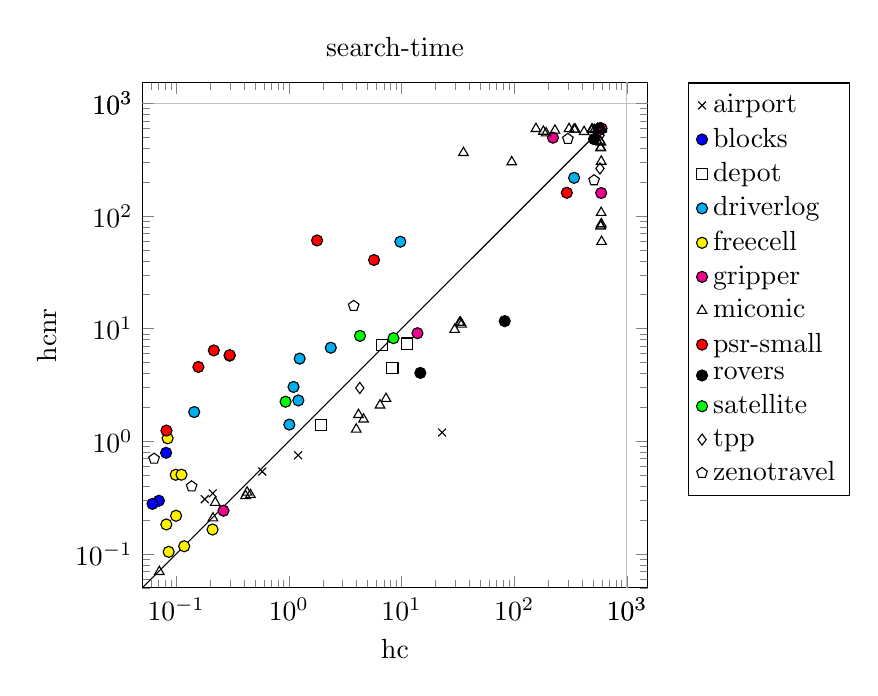
\begin{tikzpicture}
\begin{axis}[extra x tick style={grid=major}, extra x ticks=1000, extra y tick style={grid=major}, 
extra y ticks=1000, height=8cm, legend cell align=left, legend style={at={(1.4, 1)}}, title=search-time, width=8cm, xlabel=hc, xmin=0.05, xmode=log, ylabel=hcnr, ymin=0.05, ymode=log]
\addplot[color=green, mark=x, mark options={{draw=black}}, only marks] coordinates {
(0.580962, 0.539156) (22.919350, 1.197450) (1.207802, 0.751533) (0.010000, 0.010000) (0.211029, 0.344864) (0.179368, 0.306256)
};
\addlegendentry{airport}
\addplot[color=blue, mark=*, mark options={{draw=black}}, only marks] coordinates {
(0.070254, 0.296864) (0.031537, 0.132323) (0.061611, 0.278351) (0.010000, 0.015546) (0.081349, 0.790786) (0.032068, 0.459737) (0.010000, 0.022621) (0.038953, 0.506324) (0.024986, 0.185765) (0.010000, 0.019080) (0.010000, 0.010000) (0.010000, 0.045402) (0.011799, 0.083719)
};
\addlegendentry{blocks}
\addplot[color=magenta, mark=square, mark options={{draw=black}}, only marks] coordinates {
(11.217900, 7.372310) (0.010000, 0.032782) (6.757340, 7.158310) (0.010000, 0.010000) (8.306120, 4.493250) (1.943620, 1.390270)
};
\addlegendentry{depot}
\addplot[color=cyan, mark=*, mark options={{draw=black}}, only marks] coordinates {
(0.297981, 5.756450) (0.144535, 1.819230) (1.100020, 3.040280) (1.214180, 2.305950) (340.116000, 218.241000) (9.760760, 59.133700) (1.246790, 5.421790) (1.009640, 1.408210) (0.013146, 0.044778) (0.010000, 0.010000) (2.354820, 6.773570)
};
\addlegendentry{driverlog}
\addplot[color=yellow, mark=*, mark options={{draw=black}}, only marks] coordinates {
(0.099746, 0.218327) (0.210252, 0.164829) (0.042857, 0.142258) (0.013246, 0.016653) (0.117766, 0.117104) (0.099051, 0.504578) (0.083962, 1.063150) (0.010000, 0.023282) (0.037383, 0.106107) (0.141554, 0.013294) (0.081759, 0.182805) (0.111385, 0.505483) (0.025328, 0.024882) (0.085739, 0.104453)
};
\addlegendentry{freecell}
\addplot[color=magenta, mark=*, mark options={{draw=black}}, only marks] coordinates {
(0.262926, 0.241988) (220.812500, 495.988300) (596.647608, 597.565062) (569.492855, 580.212440) (0.010000, 0.010000) (13.844100, 9.110310) (591.089502, 160.080000)
};
\addlegendentry{gripper}
\addplot[color=cyan, mark=triangle, mark options={{draw=black}}, only marks] coordinates {
(339.622700, 588.378030) (0.010000, 0.011511) (549.845320, 596.864944) (590.112556, 597.189862) (7.282070, 2.391340) (0.010000, 0.012300) (0.412567, 0.327916) (584.148657, 401.133000) (6.442820, 2.091980) (0.039212, 0.046379) (3.963360, 1.277520) (590.819602, 107.059000) (586.187417, 597.268517) (306.656100, 594.349870) (95.053000, 301.677300) (34.077400, 10.919400) (181.635500, 562.785100) (0.010000, 0.012302) (35.450700, 364.431800) (594.301000, 589.966394) (592.930220, 85.041900) (585.482311, 81.044100) (0.026386, 0.042528) (570.608013, 597.167369) (347.818020, 587.793298) (155.906400, 595.750950) (32.738500, 11.323200) (596.722586, 598.978263) (0.070847, 0.069548) (191.937600, 544.281070) (577.370218, 460.882000) (496.366840, 586.208798) (0.042445, 0.049317) (592.167179, 305.104556) (0.455739, 0.335505) (29.592500, 9.804140) (0.048676, 0.049344) (4.148850, 1.722520) (585.890390, 82.624400) (0.212131, 0.208158) (586.905028, 407.188000) (577.634284, 595.238650) (588.228783, 451.849000) (517.980280, 582.901515) (0.222096, 0.285741) (488.742600, 588.815017) (596.108119, 59.254000) (229.859700, 575.452420) (4.599160, 1.569080) (0.010000, 0.010000) (33.443600, 11.359900) (0.425846, 0.352192) (417.259400, 559.410200) (0.010000, 0.012175)
};
\addlegendentry{miconic}
\addplot[color=red, mark=*, mark options={{draw=black}}, only marks] coordinates {
(0.010000, 0.011470) (0.010000, 0.032399) (293.244000, 160.887713) (0.010000, 0.012510) (0.020875, 0.200436) (0.215694, 6.411470) (0.010000, 0.019380) (0.081920, 1.245030) (0.013860, 0.108072) (0.034962, 0.448613) (0.020044, 0.175404) (0.157385, 4.569860) (0.010000, 0.044764) (0.011576, 0.024512) (0.298527, 5.820420) (0.010000, 0.010334) (0.010000, 0.058066) (1.779940, 60.661200) (0.010000, 0.020175) (0.030218, 0.282279) (0.014752, 0.078198) (0.010000, 0.010393) (0.010000, 0.031036) (0.010850, 0.076801) (0.010000, 0.015075) (0.016773, 0.031202) (0.022007, 0.111476) (0.010000, 0.010273) (0.010000, 0.010000) (5.700890, 40.694000)
};
\addlegendentry{psr-small}
\addplot[color=black, mark=*, mark options={{draw=black}}, only marks] coordinates {
(14.684900, 4.047890) (82.362900, 11.664700) (511.206762, 481.269259) (0.010000, 0.010000)
};
\addlegendentry{rovers}
\addplot[color=green, mark=*, mark options={{draw=black}}, only marks] coordinates {
(8.485640, 8.230840) (0.016291, 0.046241) (0.935294, 2.246410) (0.010000, 0.010000) (0.010000, 0.027242) (4.278860, 8.627940)
};
\addlegendentry{satellite}
\addplot[color=blue, mark=diamond, mark options={{draw=black}}, only marks] coordinates {
(578.425608, 519.404647) (4.261390, 2.976200) (0.033617, 0.096048) (576.817000, 264.094000) (0.010000, 0.010000)
};
\addlegendentry{tpp}
\addplot[color=red, mark=pentagon, mark options={{draw=black}}, only marks] coordinates {
(511.621367, 207.755000) (0.018711, 0.085917) (553.269035, 596.441548) (0.010000, 0.020608) (0.063638, 0.701225) (3.762470, 15.939800) (0.010000, 0.010000) (0.010000, 0.016045) (0.010000, 0.011999) (0.137054, 0.398511) (299.509103, 483.854610)
};
\addlegendentry{zenotravel}
\addplot[color=black] coordinates {(0.050000, 0.050000) (598, 598)};
\end{axis}
\end{tikzpicture}
\\
        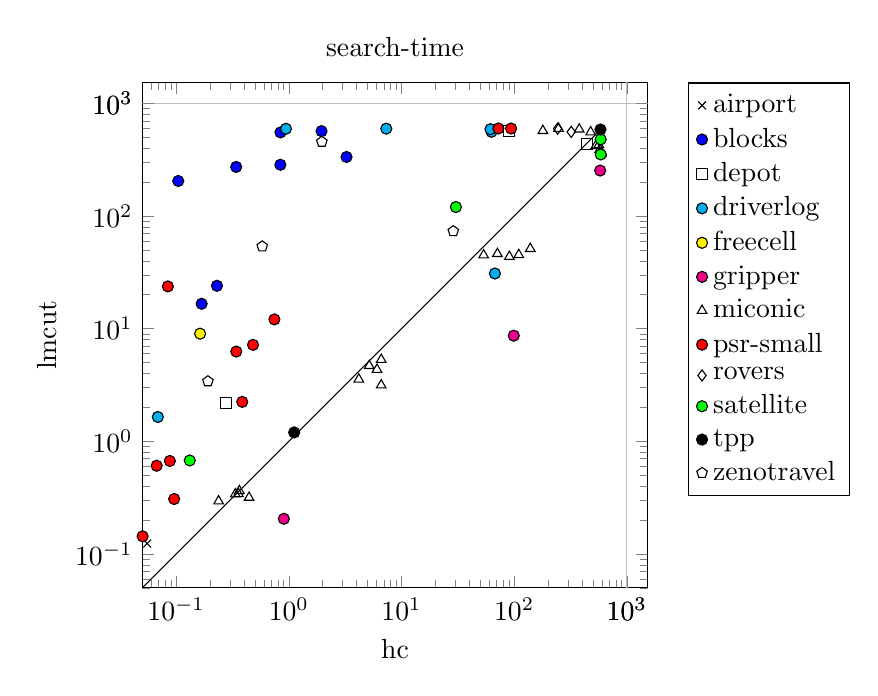
\begin{tikzpicture}
\begin{axis}[extra x tick style={grid=major}, extra x ticks=1000, extra y tick style={grid=major}, extra y ticks=1000, 
height=8.00cm, legend cell align=left, legend style={at={(1.4, 1)}}, title=search-time, width=8.00cm, xlabel=hc, xmin=0.05, xmode=log, ylabel=lmcut, ymin=0.05, ymode=log]
\addplot[color=green, mark=x, mark options={{draw=black}}, only marks] coordinates {
(0.048574, 0.120299) (0.046050, 0.111071) (0.055281, 0.123871) (0.010000, 0.010000) (0.041357, 0.108940)
};
\addlegendentry{airport}
\addplot[color=blue, mark=*, mark options={{draw=black}}, only marks] coordinates {
(0.230047, 24.030000) (0.010000, 0.031479) (0.025873, 4.558310) (0.843013, 552.542811) (0.168246, 16.629000) (0.010000, 0.027709) (0.340901, 272.692000) (1.950830, 566.580613) (3.251590, 334.247000) (0.010000, 0.362648) (0.013312, 0.390551) (0.010000, 0.062532) (0.010000, 0.010000) (0.104296, 204.640000) (0.841473, 285.099000) (0.010000, 0.228853)
};
\addlegendentry{blocks}
\addplot[color=magenta, mark=square, mark options={{draw=black}}, only marks] coordinates {
(0.278061, 2.194290) (0.010000, 0.011175) (441.957403, 437.746983) (90.623300, 571.810165)
};
\addlegendentry{depot}
\addplot[color=cyan, mark=*, mark options={{draw=black}}, only marks] coordinates {
(7.332420, 596.147586) (0.942436, 595.142993) (62.976600, 559.171837) (67.492700, 30.890800) (0.068716, 1.645040) (0.010000, 0.014424) (61.657100, 590.020191)
};
\addlegendentry{driverlog}
\addplot[color=yellow, mark=*, mark options={{draw=black}}, only marks] coordinates {
(0.163048, 9.025770)
};
\addlegendentry{freecell}
\addplot[color=magenta, mark=*, mark options={{draw=black}}, only marks] coordinates {
(0.903325, 0.205256) (580.451050, 253.325000) (0.022548, 0.015056) (99.204100, 8.665220)
};
\addlegendentry{gripper}
\addplot[color=cyan, mark=triangle, mark options={{draw=black}}, only marks] coordinates {
(576.011881, 389.226000) (71.049900, 46.231500) (564.582662, 428.204000) (0.356830, 0.341769) (477.705820, 556.250166) (53.585600, 45.017000) (90.713600, 43.600100) (0.057181, 0.048574) (179.939100, 572.062491) (139.131000, 51.293500) (0.026238, 0.041037) (0.050551, 0.046426) (0.046988, 0.047282) (593.599832, 359.371000) (0.334975, 0.339808) (247.974400, 597.565185) (6.607240, 3.151880) (0.023070, 0.038922) (0.363855, 0.363542) (0.237966, 0.294433) (109.895000, 45.257500) (6.610370, 5.314100) (378.202100, 588.854652) (0.443423, 0.316996) (6.064860, 4.336280) (5.174240, 4.686660) (4.182060, 3.551270) (531.653339, 420.967000) (0.010000, 0.010000)
};
\addlegendentry{miconic}
\addplot[color=red, mark=*, mark options={{draw=black}}, only marks] coordinates {
(0.084348, 23.722300) (93.962700, 598.190931) (0.025299, 0.938619) (0.341576, 6.263790) (0.028221, 26.004900) (0.010000, 0.048287) (0.087873, 0.668967) (0.385828, 2.239800) (0.010000, 0.021130) (0.012386, 0.062160) (0.010000, 0.011759) (0.480840, 7.183010) (0.022369, 0.994706) (0.744401, 12.090800) (0.010000, 0.012970) (0.010000, 0.020451) (0.039768, 0.225446) (0.017934, 0.042342) (0.010000, 0.010892) (0.027529, 0.049036) (72.487900, 599.024594) (0.010000, 0.017533) (0.010000, 0.025226) (0.031668, 0.130135) (0.010000, 0.021697) (0.010000, 0.014396) (0.023448, 0.093158) (0.095937, 0.307649) (0.019262, 0.219040) (0.058920, 0.030411) (0.067107, 0.607171) (0.013632, 0.866814) (0.015867, 0.823189) (0.050345, 0.143485) (0.010000, 0.010000)
};
\addlegendentry{psr-small}
\addplot[color=blue, mark=diamond, mark options={{draw=black}}, only marks] coordinates {
(243.087041, 596.896720) (0.010000, 0.018420) (321.248641, 558.373378) (0.010000, 0.031314) (0.010000, 0.010000) (0.010000, 0.017019)
};
\addlegendentry{rovers}
\addplot[color=green, mark=*, mark options={{draw=black}}, only marks] coordinates {
(30.415200, 120.126000) (0.131941, 0.676322) (0.026147, 0.120091) (586.529861, 479.144000) (587.444295, 351.926000) (0.010000, 0.010000)
};
\addlegendentry{satellite}
\addplot[color=black, mark=*, mark options={{draw=black}}, only marks] coordinates {
(0.018018, 0.022904) (1.115150, 1.199440) (583.635883, 586.030800) (0.010000, 0.010000)
};
\addlegendentry{tpp}
\addplot[color=red, mark=pentagon, mark options={{draw=black}}, only marks] coordinates {
(0.580617, 53.775400) (28.824500, 73.376400) (1.963960, 455.922727) (0.010000, 0.256246) (0.010000, 0.010000) (0.191202, 3.411590) (0.010000, 0.466716)
};
\addlegendentry{zenotravel}
\addplot[color=black] coordinates {(0.050000, 0.050000) (599, 599)};
\end{axis}
\end{tikzpicture}
\\
        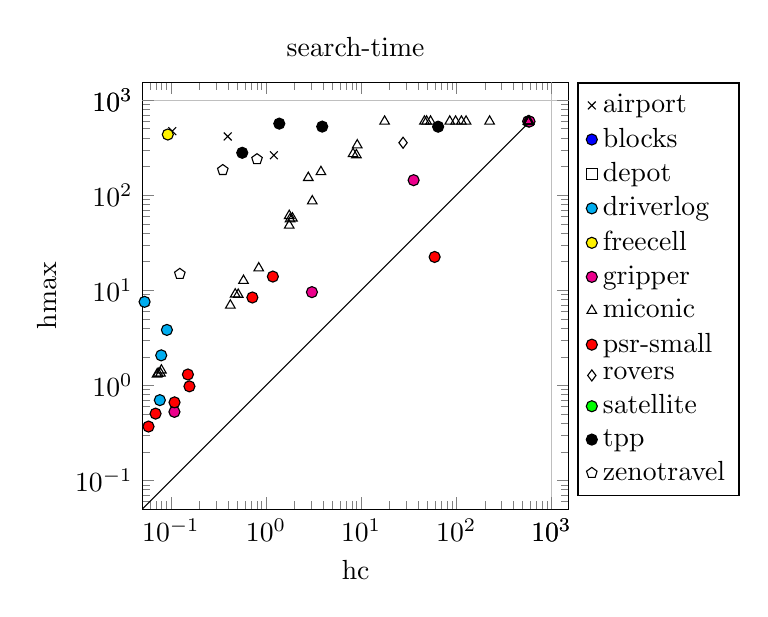
\begin{tikzpicture}
\begin{axis}[extra x tick style={grid=major}, extra x ticks=1000, extra y tick style={grid=major}, extra y ticks=1000, 
height=7.00cm, legend cell align=left, legend style={at={(1.4, 1)}}, title=search-time, width=7.00cm, xlabel=hc, xmin=0.05, xmode=log, ylabel=hmax, ymin=0.05, ymode=log]
\addplot[color=green, mark=x, mark options={{draw=black}}, only marks] coordinates {
(0.010000, 0.016491) (0.016494, 6.755030) (0.010000, 0.717950) (0.010000, 0.590599) (0.395736, 414.959000) (0.103385, 472.065000) (0.010000, 0.010000) (1.210125, 263.493000) (0.010000, 0.015102) (0.010000, 0.016054) (0.010000, 0.015509) (0.010000, 0.687614) (0.010000, 32.734900)
};
\addlegendentry{airport}
\addplot[color=blue, mark=*, mark options={{draw=black}}, only marks] coordinates {
(0.021018, 0.372409) (0.010000, 0.050527) (0.012726, 0.308366) (0.010000, 0.066047) (0.010000, 0.019459) (0.010430, 0.241785) (0.020812, 0.344101) (0.010000, 0.020340) (0.021315, 0.474589) (0.010446, 0.194772) (0.010000, 0.010000) (0.010000, 0.066848) (0.010000, 0.018284)
};
\addlegendentry{blocks}
\addplot[color=magenta, mark=square, mark options={{draw=black}}, only marks] coordinates {
(0.010000, 0.031612) (0.044016, 9.777910) (0.010000, 0.459406) (0.010000, 0.010000) (0.018111, 1.893310) (0.011065, 0.716715)
};
\addlegendentry{depot}
\addplot[color=cyan, mark=*, mark options={{draw=black}}, only marks] coordinates {
(0.079113, 2.071450) (0.011772, 0.146100) (0.010000, 0.010000) (0.010000, 0.038347) (0.012175, 0.432243) (0.090763, 3.835300) (0.042196, 1.016020) (0.076491, 0.700432) (0.022317, 0.523188) (0.052872, 7.568230) (0.029184, 1.031880)
};
\addlegendentry{driverlog}
\addplot[color=yellow, mark=*, mark options={{draw=black}}, only marks] coordinates {
(0.025467, 543.707805) (0.010000, 7.079400) (0.010000, 342.542000) (0.010000, 1.322830) (0.017503, 54.521000) (0.010000, 163.241000) (0.047170, 264.016000) (0.010000, 1.283090) (0.033165, 152.929000) (0.010000, 1.461090) (0.010114, 34.483100) (0.010000, 98.255600) (0.012825, 443.515000) (0.010000, 0.524055) (0.010000, 68.535000) (0.010000, 0.520173) (0.010000, 0.523277) (0.010508, 235.652000) (0.010000, 0.446854) (0.010000, 6.151280) (0.010000, 1.360380) (0.010000, 238.460000) (0.010000, 1.073300) (0.031360, 438.364005) (0.044098, 526.096000) (0.037899, 517.092605) (0.014858, 516.261105) (0.092770, 435.115005) (0.010000, 1.437480) (0.029469, 148.491000) (0.010000, 0.190178) (0.010000, 8.337660) (0.010000, 7.290870) (0.010000, 0.523382) (0.010000, 0.067749) (0.027610, 448.797605) (0.010000, 321.654000) (0.010000, 6.312610) (0.010000, 6.952450) (0.015431, 493.080105) (0.010135, 44.046300) (0.010000, 0.519870) (0.030210, 464.824105)
};
\addlegendentry{freecell}
\addplot[color=magenta, mark=*, mark options={{draw=black}}, only marks] coordinates {
(0.108904, 0.527269) (0.010000, 0.053869) (35.658600, 144.022000) (580.503765, 598.073514) (3.040280, 9.573330) (0.010000, 0.010000) (570.510251, 598.167887) (589.880727, 596.319431)
};
\addlegendentry{gripper}
\addplot[color=cyan, mark=triangle, mark options={{draw=black}}, only marks] coordinates {
(224.446000, 597.933579) (0.510274, 9.035710) (573.474019, 597.365275) (1.788500, 56.040000) (8.228750, 272.530000) (0.579897, 12.645000) (0.021994, 0.305318) (0.010000, 0.013467) (1.897180, 57.236000) (9.107240, 336.694000) (0.073420, 1.336390) (583.477356, 599.408217) (0.474537, 9.099500) (0.010000, 0.054482) (0.010000, 0.020015) (0.010000, 0.019408) (569.532000, 597.087791) (0.079419, 1.444580) (48.852000, 597.974743) (126.919000, 598.062657) (2.784220, 152.824000) (1.754290, 48.142100) (113.458000, 597.760290) (0.010899, 0.074368) (85.522600, 597.865548) (0.010000, 0.019519) (98.525400, 597.754485) (0.019884, 0.260593) (53.705700, 597.862635) (0.010000, 0.010000) (8.918480, 264.814000) (577.266961, 592.260441) (0.011328, 0.066050) (0.010000, 0.052879) (579.359401, 596.516783) (577.410498, 596.063198) (17.665800, 597.651457) (3.781750, 176.252000) (0.838683, 17.129900) (0.011444, 0.070371) (0.010000, 0.019296) (0.071420, 1.306580) (0.077724, 1.337580) (0.019188, 0.208439) (0.421684, 6.954340) (0.034272, 0.414753) (3.065430, 86.787300) (0.041777, 0.485996) (46.340500, 598.207505) (1.755410, 60.925600)
};
\addlegendentry{miconic}
\addplot[color=red, mark=*, mark options={{draw=black}}, only marks] coordinates {
(0.010000, 0.030722) (0.010000, 0.057003) (0.010000, 0.013188) (0.015711, 0.135814) (0.014667, 0.102157) (0.010000, 0.010121) (0.010000, 0.018390) (0.718811, 8.410160) (0.010000, 0.036949) (0.010000, 0.016502) (0.150947, 1.303090) (0.010000, 0.038536) (0.010000, 0.021252) (0.015564, 0.141229) (0.068998, 0.505190) (0.019144, 0.093764) (0.010534, 0.043708) (0.156583, 0.977566) (0.010000, 0.044692) (1.180550, 13.957400) (0.058158, 0.369399) (0.013244, 0.051112) (0.010000, 0.015697) (0.010000, 0.058230) (0.109162, 0.663662) (0.010000, 0.010000) (59.320100, 22.437753)
};
\addlegendentry{psr-small}
\addplot[color=blue, mark=diamond, mark options={{draw=black}}, only marks] coordinates {
(0.019173, 0.293917) (27.633300, 356.412000) (0.044183, 0.495889) (0.010000, 0.010000)
};
\addlegendentry{rovers}
\addplot[color=green, mark=*, mark options={{draw=black}}, only marks] coordinates {
(0.010000, 0.013571) (0.010000, 0.010000) (0.021058, 1.343910) (0.031887, 12.418500) (0.010000, 0.014210) (0.019496, 0.882318)
};
\addlegendentry{satellite}
\addplot[color=black, mark=*, mark options={{draw=black}}, only marks] coordinates {
(3.901330, 526.821972) (0.010000, 0.015316) (0.044292, 10.255400) (0.010000, 0.359451) (1.379290, 566.276805) (0.010000, 0.010000) (0.562574, 279.485000) (64.543100, 525.581644)
};
\addlegendentry{tpp}
\addplot[color=red, mark=pentagon, mark options={{draw=black}}, only marks] coordinates {
(0.014180, 0.211603) (0.032232, 3.192170) (0.010000, 0.020350) (0.010000, 0.012913) (0.010000, 0.027564) (0.804290, 239.404000) (0.124137, 14.887400) (0.010000, 0.010000) (0.351318, 184.058000) (0.010000, 0.077096) (0.010000, 0.016207)
};
\addlegendentry{zenotravel}
\addplot[color=black] coordinates {(0.050000, 0.050000) (599, 599)};
\end{axis}
\end{tikzpicture}
\\
        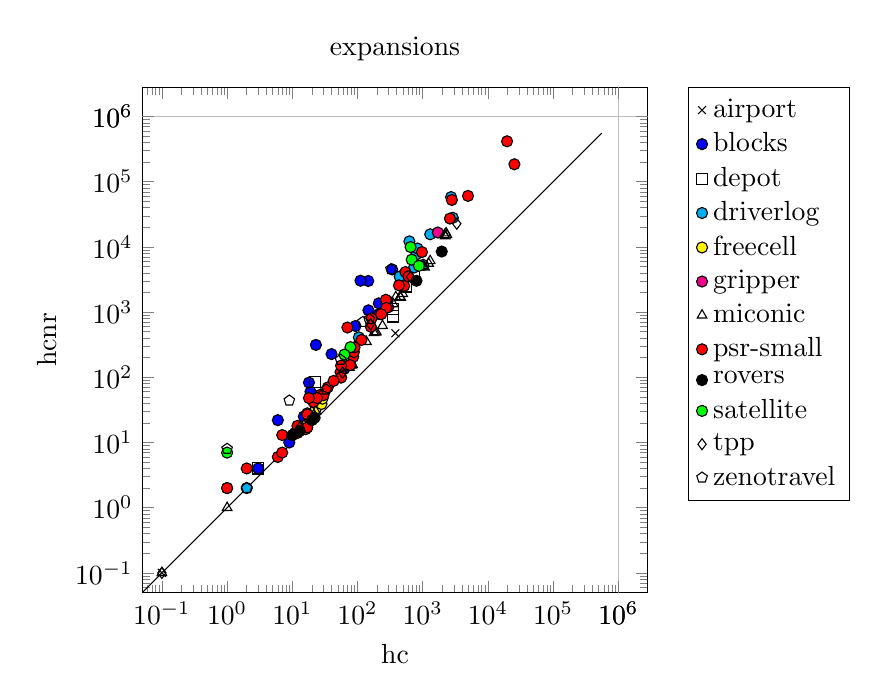
\begin{tikzpicture}
\begin{axis}[extra x tick style={grid=major}, extra x ticks=1000000, extra y tick style={grid=major}, extra y ticks=1000000, 
height=8cm, legend cell align=left, legend style={at={(1.4, 1)}}, title=expansions, width=8.00cm, xlabel=hc, xmin=0.05, xmode=log, ylabel=hcnr, ymin=0.05, ymode=log]
\addplot[color=green, mark=x, mark options={{draw=black}}, only marks] coordinates {
(381, 473) (0.100000, 0.100000) (18, 18)
};
\addlegendentry{airport}
\addplot[color=blue, mark=*, mark options={{draw=black}}, only marks] coordinates {
(1, 2) (40, 227) (147, 1065) (19, 60) (63, 135) (146, 3001) (15, 25) (3, 4) (93, 611) (111, 3029) (340, 4510) (213, 931) (9, 10) (18, 83) (23, 314) (6, 22) (212, 1362) (289, 1470)
};
\addlegendentry{blocks}
\addplot[color=magenta, mark=square, mark options={{draw=black}}, only marks] coordinates {
(22, 84) (347, 858) (352, 1102) (551, 2477) (3, 4) (729, 3670)
};
\addlegendentry{depot}
\addplot[color=cyan, mark=*, mark options={{draw=black}}, only marks] coordinates {
(105, 410) (793, 7645) (835, 9442) (737, 4825) (1304, 15612) (2896, 27945) (1017, 5306) (625, 12152) (2, 2) (2726, 58064) (443, 3510)
};
\addlegendentry{driverlog}
\addplot[color=yellow, mark=*, mark options={{draw=black}}, only marks] coordinates {
(17, 19) (17, 28) (23, 33) (28, 39) (29, 47)
};
\addlegendentry{freecell}
\addplot[color=magenta, mark=*, mark options={{draw=black}}, only marks] coordinates {
(1707, 16634) (296, 1188) (56, 100)
};
\addlegendentry{gripper}
\addplot[color=cyan, mark=triangle, mark options={{draw=black}}, only marks] coordinates {
(20, 25) (1233, 5566) (0.100000, 0.100000) (82, 156) (460, 1675) (137, 351) (449, 1726) (23, 30) (54, 106) (20, 30) (1028, 4987) (84, 156) (1025, 5152) (179, 481) (242, 619) (1, 1) (1302, 6110) (2228, 14732) (187, 488) (493, 1916) (386, 1711) (2159, 15261) (2352, 15271) (195, 495) (22, 25) (1069, 4857) (354, 1334) (80, 153) (2282, 16310) (19, 25) (75, 141)
};
\addlegendentry{miconic}
\addplot[color=red, mark=*, mark options={{draw=black}}, only marks] coordinates {
(19675, 416544) (78, 156) (974, 8330) (160, 597) (115, 374) (6, 6) (272, 1545) (22, 44) (7, 7) (2614, 27214) (277, 1161) (16, 16) (21, 42) (11, 14) (521, 2527) (55, 120) (4955, 60566) (1, 2) (543, 4117) (59, 149) (86, 206) (602, 3537) (27, 54) (88, 244) (70, 580) (12, 14) (30, 53) (18, 24) (24, 48) (77, 154) (12, 18) (56, 151) (17, 27) (35, 70) (231, 928) (18, 48) (90, 288) (7, 13) (2800, 52482) (17, 17) (56, 99) (25480, 185128) (43, 88) (164, 801) (2, 4) (432, 2572)
};
\addlegendentry{psr-small}
\addplot[color=black, mark=*, mark options={{draw=black}}, only marks] coordinates {
(22, 24) (10, 13) (13, 15) (1960, 8490) (803, 3022) (20, 22)
};
\addlegendentry{rovers}
\addplot[color=green, mark=*, mark options={{draw=black}}, only marks] coordinates {
(652, 9941) (678, 6371) (876, 5124) (1, 7) (78, 290) (63, 223)
};
\addlegendentry{satellite}
\addplot[color=blue, mark=diamond, mark options={{draw=black}}, only marks] coordinates {
(3331, 22681) (649, 3465) (158, 648) (13, 17) (0.100000, 0.100000) (59, 118)
};
\addlegendentry{tpp}
\addplot[color=red, mark=pentagon, mark options={{draw=black}}, only marks] coordinates {
(121, 708) (1, 8) (55, 186) (2, 2) (151, 780) (326, 4556) (33, 65) (9, 44)
};
\addlegendentry{zenotravel}
\addplot[color=black] coordinates {(0.050000, 0.050000) (556807, 556807)};
\end{axis}
\end{tikzpicture}
\\
        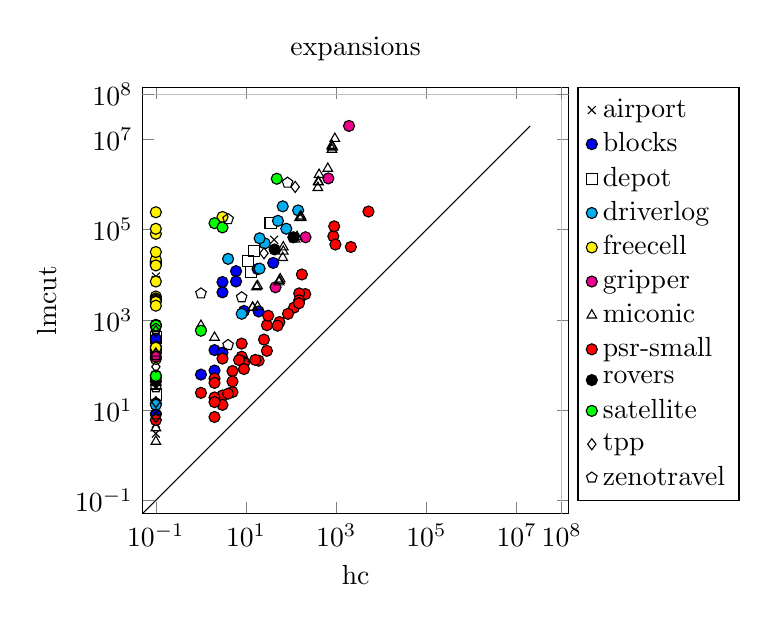
\begin{tikzpicture}
\begin{axis}[extra x tick style={grid=major}, extra x ticks=100000000, extra y tick style={grid=major}, extra y ticks=100000000, 
height=7.00cm, legend cell align=left, legend style={at={(1.4, 1)}}, title=expansions, width=7.00cm, xlabel=hc, xmin=0.05, xmode=log, ylabel=lmcut, ymin=0.05, ymode=log]
\addplot[color=green, mark=x, mark options={{draw=black}}, only marks] coordinates {
(0.100000, 33) (0.100000, 219) (0.100000, 181) (42, 59492) (0.100000, 217) (0.100000, 6) (0.100000, 9131) (0.100000, 5) (0.100000, 7615) (0.100000, 7625) (0.100000, 245) (0.100000, 3) (0.100000, 8)
};
\addlegendentry{airport}
\addplot[color=blue, mark=*, mark options={{draw=black}}, only marks] coordinates {
(18, 13376) (0.100000, 187) (2, 213) (6, 12007) (0.100000, 58) (6, 7076) (9, 1570) (0.100000, 14) (19, 1532) (3, 4066) (2, 75) (0.100000, 379) (3, 6886) (40, 18268) (1, 61) (0.100000, 8) (3, 187)
};
\addlegendentry{blocks}
\addplot[color=magenta, mark=square, mark options={{draw=black}}, only marks] coordinates {
(0.100000, 22) (15, 34039) (11, 20162) (35, 142452) (13, 11292) (0.100000, 407)
};
\addlegendentry{depot}
\addplot[color=cyan, mark=*, mark options={{draw=black}}, only marks] coordinates {
(0.100000, 16896) (26, 49620) (20, 64248) (51, 156560) (0.100000, 13) (143, 266848) (4, 22448) (65, 328115) (20, 13650) (8, 1360) (78, 104720)
};
\addlegendentry{driverlog}
\addplot[color=yellow, mark=*, mark options={{draw=black}}, only marks] coordinates {
(0.100000, 17761) (0.100000, 3286) (0.100000, 2971) (0.100000, 7067) (0.100000, 19591) (0.100000, 242704) (0.100000, 19141) (0.100000, 21631) (0.100000, 226) (0.100000, 136) (0.100000, 211) (0.100000, 2791) (3, 190470) (0.100000, 2626) (0.100000, 256) (0.100000, 16051) (0.100000, 241) (0.100000, 2506) (0.100000, 80809) (0.100000, 2056) (0.100000, 31823) (0.100000, 766) (0.100000, 104311)
};
\addlegendentry{freecell}
\addplot[color=magenta, mark=*, mark options={{draw=black}}, only marks] coordinates {
(1920, 19916814) (45, 5268) (208, 67710) (0.100000, 151) (668, 1367176)
};
\addlegendentry{gripper}
\addplot[color=cyan, mark=triangle, mark options={{draw=black}}, only marks] coordinates {
(55, 7443) (0.100000, 181) (135, 69039) (155, 185047) (18, 5647) (819, 6915236) (156, 182083) (0.100000, 43) (2, 406) (395, 1143604) (409, 1131564) (17, 5356) (824, 6718966) (803, 5972930) (54, 6872) (18, 1954) (14, 1892) (416, 1656749) (0.100000, 50) (67, 40958) (0.100000, 4) (122, 60879) (57, 8012) (65, 23797) (166, 185293) (391, 846923) (931, 10411953) (649, 2261005) (14, 1861) (801, 7337121) (164, 198138) (1, 745) (0.100000, 2) (67, 32915)
};
\addlegendentry{miconic}
\addplot[color=red, mark=*, mark options={{draw=black}}, only marks] coordinates {
(5, 73) (206, 3719) (863, 71216) (902, 118208) (3, 21) (29, 760) (8, 152) (19, 124) (958, 46688) (9, 116) (116, 1866) (55, 892) (151, 3851) (3, 138) (31, 1232) (25, 364) (8, 297) (5, 25) (4, 23) (0.100000, 772) (9, 109) (173, 10124) (3, 13) (2109, 41214) (29, 205) (5183, 251714) (85, 1355) (1, 24) (2, 19) (2, 7) (151, 2707) (7, 128) (2, 50) (2, 40) (5, 43) (16, 129) (0.100000, 6) (9, 81) (2, 15) (50, 741) (149, 2328)
};
\addlegendentry{psr-small}
\addplot[color=black, mark=*, mark options={{draw=black}}, only marks] coordinates {
(43, 36383) (0.100000, 43) (0.100000, 50) (112, 67588)
};
\addlegendentry{rovers}
\addplot[color=green, mark=*, mark options={{draw=black}}, only marks] coordinates {
(0.100000, 57) (2, 138858) (48, 1342395) (0.100000, 745) (1, 573) (3, 112017)
};
\addlegendentry{satellite}
\addplot[color=blue, mark=diamond, mark options={{draw=black}}, only marks] coordinates {
(0.100000, 91) (0.100000, 15) (0.100000, 559) (0.100000, 7) (25, 29953) (123, 884427)
};
\addlegendentry{tpp}
\addplot[color=red, mark=pentagon, mark options={{draw=black}}, only marks] coordinates {
(0.100000, 8) (0.100000, 632) (1, 3844) (0.100000, 166) (4, 170892) (8, 3160) (83, 1096013) (0.100000, 32) (4, 276)
};
\addlegendentry{zenotravel}
\addplot[color=black] coordinates {(0.050000, 0.050000) (19916814, 19916814)};
\end{axis}
\end{tikzpicture}
\\
        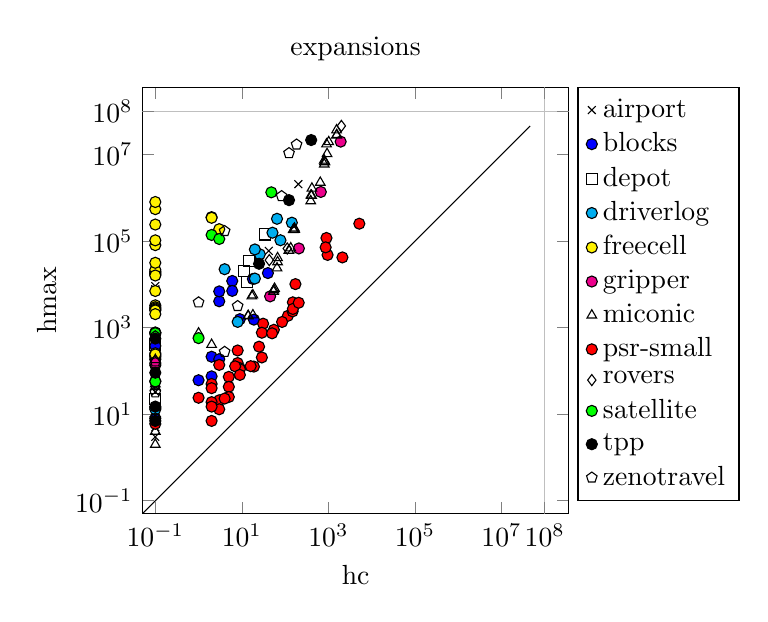
\begin{tikzpicture}
\begin{axis}[extra x tick style={grid=major}, extra x ticks=100000000, extra y tick style={grid=major}, extra y ticks=100000000, 
height=7.00cm, legend cell align=left, legend style={at={(1.4, 1)}}, title=expansions, width=7.00cm, xlabel=hc, xmin=0.05, xmode=log, ylabel=hmax, ymin=0.05, ymode=log]
\addplot[color=green, mark=x, mark options={{draw=black}}, only marks] coordinates {
(42, 59583) (0.100000, 33) (0.100000, 219) (0.100000, 181) (0.100000, 6) (0.100000, 217) (0.100000, 245) (202, 2073240) (0.100000, 9131) (0.100000, 5) (0.100000, 7615) (0.100000, 7625) (0.100000, 3) (0.100000, 8)
};
\addlegendentry{airport}
\addplot[color=blue, mark=*, mark options={{draw=black}}, only marks] coordinates {
(9, 1572) (18, 13376) (0.100000, 379) (6, 12007) (0.100000, 58) (6, 7076) (0.100000, 14) (2, 213) (3, 4066) (2, 75) (0.100000, 187) (40, 18270) (3, 6886) (1, 61) (0.100000, 8) (3, 187) (19, 1534)
};
\addlegendentry{blocks}
\addplot[color=magenta, mark=square, mark options={{draw=black}}, only marks] coordinates {
(0.100000, 22) (35, 142466) (13, 11292) (11, 20161) (15, 34032) (0.100000, 407)
};
\addlegendentry{depot}
\addplot[color=cyan, mark=*, mark options={{draw=black}}, only marks] coordinates {
(0.100000, 16896) (26, 49620) (20, 64248) (51, 156560) (0.100000, 13) (143, 266816) (4, 22448) (20, 13650) (8, 1360) (65, 328078) (78, 104720)
};
\addlegendentry{driverlog}
\addplot[color=yellow, mark=*, mark options={{draw=black}}, only marks] coordinates {
(0.100000, 17761) (0.100000, 3286) (0.100000, 2971) (0.100000, 19591) (2, 357856) (0.100000, 19141) (0.100000, 548746) (0.100000, 21631) (0.100000, 226) (0.100000, 136) (0.100000, 802036) (0.100000, 211) (0.100000, 2791) (0.100000, 31561) (0.100000, 2626) (0.100000, 7036) (0.100000, 256) (0.100000, 16051) (0.100000, 241) (0.100000, 80806) (0.100000, 2506) (0.100000, 2056) (2, 346276) (3, 188791) (0.100000, 766) (0.100000, 104311) (0.100000, 241546)
};
\addlegendentry{freecell}
\addplot[color=magenta, mark=*, mark options={{draw=black}}, only marks] coordinates {
(1920, 19918398) (668, 1368076) (208, 67738) (0.100000, 151) (45, 5283)
};
\addlegendentry{gripper}
\addplot[color=cyan, mark=triangle, mark options={{draw=black}}, only marks] coordinates {
(395, 1143601) (0.100000, 181) (18, 5647) (409, 1131640) (0.100000, 43) (801, 7341225) (17, 5356) (1563, 28711853) (67, 40955) (391, 846921) (931, 10420707) (18, 1954) (803, 5975018) (55, 7441) (0.100000, 50) (907, 17460317) (122, 60875) (1019, 19611126) (156, 182080) (166, 185292) (819, 6917972) (155, 185045) (1542, 36749162) (65, 23798) (54, 6870) (824, 6722843) (0.100000, 4) (1545, 27889713) (649, 2261740) (14, 1861) (416, 1656947) (67, 32916) (57, 8012) (2, 406) (1, 745) (14, 1892) (164, 198133) (135, 69035) (0.100000, 2)
};
\addlegendentry{miconic}
\addplot[color=red, mark=*, mark options={{draw=black}}, only marks] coordinates {
(116, 1880) (5, 73) (902, 118208) (3, 21) (173, 10156) (8, 152) (2, 19) (9, 116) (5, 43) (55, 892) (151, 3851) (3, 138) (25, 364) (8, 297) (5, 25) (4, 23) (149, 2378) (5183, 252962) (0.100000, 772) (31, 1236) (958, 47992) (9, 109) (1, 24) (3, 13) (29, 764) (2109, 42030) (29, 205) (85, 1355) (19, 126) (2, 7) (151, 2707) (7, 128) (2, 50) (863, 71716) (2, 40) (16, 129) (0.100000, 6) (206, 3759) (9, 81) (2, 15) (50, 741)
};
\addlegendentry{psr-small}
\addplot[color=blue, mark=diamond, mark options={{draw=black}}, only marks] coordinates {
(0.100000, 43) (112, 67588) (43, 36387) (1997, 45935775) (0.100000, 50)
};
\addlegendentry{rovers}
\addplot[color=green, mark=*, mark options={{draw=black}}, only marks] coordinates {
(0.100000, 57) (48, 1342391) (2, 138858) (0.100000, 745) (1, 573) (3, 112017)
};
\addlegendentry{satellite}
\addplot[color=black, mark=*, mark options={{draw=black}}, only marks] coordinates {
(0.100000, 91) (0.100000, 559) (0.100000, 15) (400, 21653693) (0.100000, 7) (123, 884552) (25, 29955)
};
\addlegendentry{tpp}
\addplot[color=red, mark=pentagon, mark options={{draw=black}}, only marks] coordinates {
(0.100000, 8) (123, 10801620) (83, 1096038) (8, 3160) (0.100000, 632) (1, 3844) (0.100000, 166) (4, 170892) (0.100000, 32) (4, 276) (184, 17075893)
};
\addlegendentry{zenotravel}
\addplot[color=black] coordinates {(0.050000, 0.050000) (45935775, 45935775)};
\end{axis}
\end{tikzpicture}

    \end{center}
   

    \subsubsection*{Cost Bound 0.5}

    \begin{center}

        \begin{tabular}{l|r|r|r|r}
            Finished PPD1 & hc & hcnr & hmax & lmcut \\\hline
            airport (19) & 12 & 12 & \textbf{16} & 15\\\hline
            blocks (18) & 18 & 18 & 18 & 18 \\\hline
            depot (6) & \textbf{6} & \textbf{6} & 5 & 4 \\\hline
            driverlog (11) & \textbf{11} & \textbf{11} & 9 & 8 \\\hline
            freecell (55) & 6 & 7 & \textbf{15} & 14 \\\hline
            gripper (8) & 3 & \textbf{4} & \textbf{4} & \textbf{4} \\\hline
            miconic (69) & 39 & \textbf{48} & 43 & 39 \\\hline
            PSR (49) & \textbf{49} & 48 & 48 & 47 \\\hline
            rovers (7) & 6 & 6 & 6 & 6 \\\hline
            satellite (6) & \textbf{6} & \textbf{6} & \textbf{6} & 4 \\\hline
            tpp (10) & \textbf{6} & \textbf{6} & 5 & 5 \\\hline
            zenotravel (11) & 8 & \textbf{9} & 7 & 7 \\\hline\hline
            sum (269) & 170 & 181 & \textbf{182} & 171 \\
        \end{tabular}

        \scriptsize
        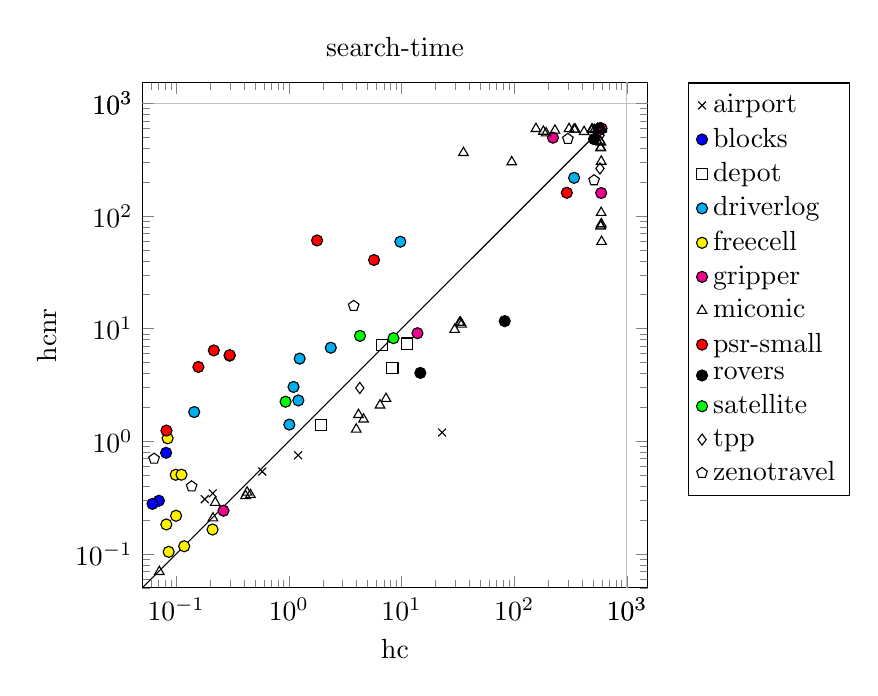
\begin{tikzpicture}
\begin{axis}[extra x tick style={grid=major}, extra x ticks=1000, extra y tick style={grid=major}, 
extra y ticks=1000, height=8cm, legend cell align=left, legend style={at={(1.4, 1)}}, title=search-time, width=8cm, xlabel=hc, xmin=0.05, xmode=log, ylabel=hcnr, ymin=0.05, ymode=log]
\addplot[color=green, mark=x, mark options={{draw=black}}, only marks] coordinates {
(0.580962, 0.539156) (22.919350, 1.197450) (1.207802, 0.751533) (0.010000, 0.010000) (0.211029, 0.344864) (0.179368, 0.306256)
};
\addlegendentry{airport}
\addplot[color=blue, mark=*, mark options={{draw=black}}, only marks] coordinates {
(0.070254, 0.296864) (0.031537, 0.132323) (0.061611, 0.278351) (0.010000, 0.015546) (0.081349, 0.790786) (0.032068, 0.459737) (0.010000, 0.022621) (0.038953, 0.506324) (0.024986, 0.185765) (0.010000, 0.019080) (0.010000, 0.010000) (0.010000, 0.045402) (0.011799, 0.083719)
};
\addlegendentry{blocks}
\addplot[color=magenta, mark=square, mark options={{draw=black}}, only marks] coordinates {
(11.217900, 7.372310) (0.010000, 0.032782) (6.757340, 7.158310) (0.010000, 0.010000) (8.306120, 4.493250) (1.943620, 1.390270)
};
\addlegendentry{depot}
\addplot[color=cyan, mark=*, mark options={{draw=black}}, only marks] coordinates {
(0.297981, 5.756450) (0.144535, 1.819230) (1.100020, 3.040280) (1.214180, 2.305950) (340.116000, 218.241000) (9.760760, 59.133700) (1.246790, 5.421790) (1.009640, 1.408210) (0.013146, 0.044778) (0.010000, 0.010000) (2.354820, 6.773570)
};
\addlegendentry{driverlog}
\addplot[color=yellow, mark=*, mark options={{draw=black}}, only marks] coordinates {
(0.099746, 0.218327) (0.210252, 0.164829) (0.042857, 0.142258) (0.013246, 0.016653) (0.117766, 0.117104) (0.099051, 0.504578) (0.083962, 1.063150) (0.010000, 0.023282) (0.037383, 0.106107) (0.141554, 0.013294) (0.081759, 0.182805) (0.111385, 0.505483) (0.025328, 0.024882) (0.085739, 0.104453)
};
\addlegendentry{freecell}
\addplot[color=magenta, mark=*, mark options={{draw=black}}, only marks] coordinates {
(0.262926, 0.241988) (220.812500, 495.988300) (596.647608, 597.565062) (569.492855, 580.212440) (0.010000, 0.010000) (13.844100, 9.110310) (591.089502, 160.080000)
};
\addlegendentry{gripper}
\addplot[color=cyan, mark=triangle, mark options={{draw=black}}, only marks] coordinates {
(339.622700, 588.378030) (0.010000, 0.011511) (549.845320, 596.864944) (590.112556, 597.189862) (7.282070, 2.391340) (0.010000, 0.012300) (0.412567, 0.327916) (584.148657, 401.133000) (6.442820, 2.091980) (0.039212, 0.046379) (3.963360, 1.277520) (590.819602, 107.059000) (586.187417, 597.268517) (306.656100, 594.349870) (95.053000, 301.677300) (34.077400, 10.919400) (181.635500, 562.785100) (0.010000, 0.012302) (35.450700, 364.431800) (594.301000, 589.966394) (592.930220, 85.041900) (585.482311, 81.044100) (0.026386, 0.042528) (570.608013, 597.167369) (347.818020, 587.793298) (155.906400, 595.750950) (32.738500, 11.323200) (596.722586, 598.978263) (0.070847, 0.069548) (191.937600, 544.281070) (577.370218, 460.882000) (496.366840, 586.208798) (0.042445, 0.049317) (592.167179, 305.104556) (0.455739, 0.335505) (29.592500, 9.804140) (0.048676, 0.049344) (4.148850, 1.722520) (585.890390, 82.624400) (0.212131, 0.208158) (586.905028, 407.188000) (577.634284, 595.238650) (588.228783, 451.849000) (517.980280, 582.901515) (0.222096, 0.285741) (488.742600, 588.815017) (596.108119, 59.254000) (229.859700, 575.452420) (4.599160, 1.569080) (0.010000, 0.010000) (33.443600, 11.359900) (0.425846, 0.352192) (417.259400, 559.410200) (0.010000, 0.012175)
};
\addlegendentry{miconic}
\addplot[color=red, mark=*, mark options={{draw=black}}, only marks] coordinates {
(0.010000, 0.011470) (0.010000, 0.032399) (293.244000, 160.887713) (0.010000, 0.012510) (0.020875, 0.200436) (0.215694, 6.411470) (0.010000, 0.019380) (0.081920, 1.245030) (0.013860, 0.108072) (0.034962, 0.448613) (0.020044, 0.175404) (0.157385, 4.569860) (0.010000, 0.044764) (0.011576, 0.024512) (0.298527, 5.820420) (0.010000, 0.010334) (0.010000, 0.058066) (1.779940, 60.661200) (0.010000, 0.020175) (0.030218, 0.282279) (0.014752, 0.078198) (0.010000, 0.010393) (0.010000, 0.031036) (0.010850, 0.076801) (0.010000, 0.015075) (0.016773, 0.031202) (0.022007, 0.111476) (0.010000, 0.010273) (0.010000, 0.010000) (5.700890, 40.694000)
};
\addlegendentry{psr-small}
\addplot[color=black, mark=*, mark options={{draw=black}}, only marks] coordinates {
(14.684900, 4.047890) (82.362900, 11.664700) (511.206762, 481.269259) (0.010000, 0.010000)
};
\addlegendentry{rovers}
\addplot[color=green, mark=*, mark options={{draw=black}}, only marks] coordinates {
(8.485640, 8.230840) (0.016291, 0.046241) (0.935294, 2.246410) (0.010000, 0.010000) (0.010000, 0.027242) (4.278860, 8.627940)
};
\addlegendentry{satellite}
\addplot[color=blue, mark=diamond, mark options={{draw=black}}, only marks] coordinates {
(578.425608, 519.404647) (4.261390, 2.976200) (0.033617, 0.096048) (576.817000, 264.094000) (0.010000, 0.010000)
};
\addlegendentry{tpp}
\addplot[color=red, mark=pentagon, mark options={{draw=black}}, only marks] coordinates {
(511.621367, 207.755000) (0.018711, 0.085917) (553.269035, 596.441548) (0.010000, 0.020608) (0.063638, 0.701225) (3.762470, 15.939800) (0.010000, 0.010000) (0.010000, 0.016045) (0.010000, 0.011999) (0.137054, 0.398511) (299.509103, 483.854610)
};
\addlegendentry{zenotravel}
\addplot[color=black] coordinates {(0.050000, 0.050000) (598, 598)};
\end{axis}
\end{tikzpicture}
\\
        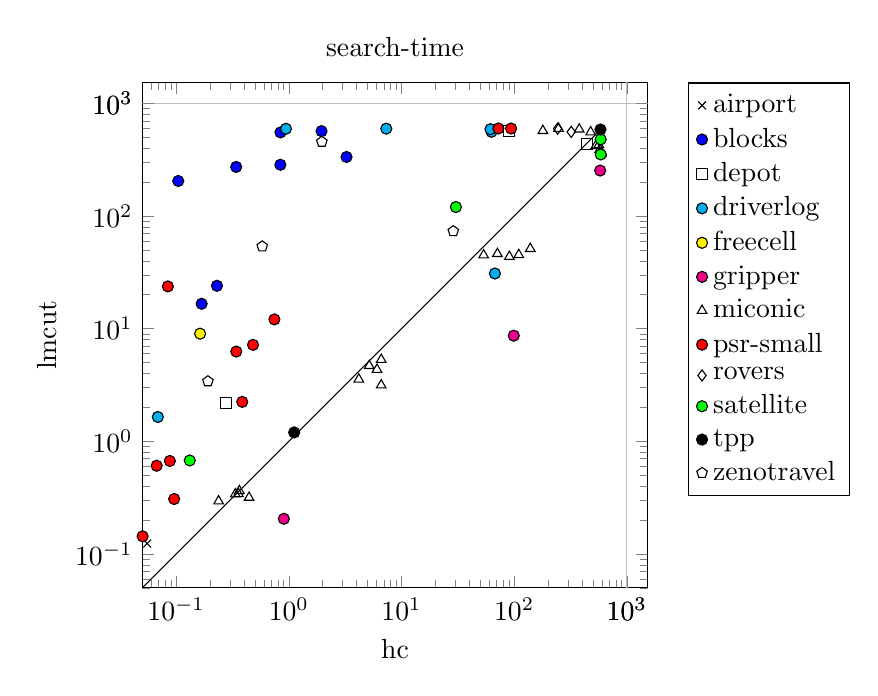
\begin{tikzpicture}
\begin{axis}[extra x tick style={grid=major}, extra x ticks=1000, extra y tick style={grid=major}, extra y ticks=1000, 
height=8.00cm, legend cell align=left, legend style={at={(1.4, 1)}}, title=search-time, width=8.00cm, xlabel=hc, xmin=0.05, xmode=log, ylabel=lmcut, ymin=0.05, ymode=log]
\addplot[color=green, mark=x, mark options={{draw=black}}, only marks] coordinates {
(0.048574, 0.120299) (0.046050, 0.111071) (0.055281, 0.123871) (0.010000, 0.010000) (0.041357, 0.108940)
};
\addlegendentry{airport}
\addplot[color=blue, mark=*, mark options={{draw=black}}, only marks] coordinates {
(0.230047, 24.030000) (0.010000, 0.031479) (0.025873, 4.558310) (0.843013, 552.542811) (0.168246, 16.629000) (0.010000, 0.027709) (0.340901, 272.692000) (1.950830, 566.580613) (3.251590, 334.247000) (0.010000, 0.362648) (0.013312, 0.390551) (0.010000, 0.062532) (0.010000, 0.010000) (0.104296, 204.640000) (0.841473, 285.099000) (0.010000, 0.228853)
};
\addlegendentry{blocks}
\addplot[color=magenta, mark=square, mark options={{draw=black}}, only marks] coordinates {
(0.278061, 2.194290) (0.010000, 0.011175) (441.957403, 437.746983) (90.623300, 571.810165)
};
\addlegendentry{depot}
\addplot[color=cyan, mark=*, mark options={{draw=black}}, only marks] coordinates {
(7.332420, 596.147586) (0.942436, 595.142993) (62.976600, 559.171837) (67.492700, 30.890800) (0.068716, 1.645040) (0.010000, 0.014424) (61.657100, 590.020191)
};
\addlegendentry{driverlog}
\addplot[color=yellow, mark=*, mark options={{draw=black}}, only marks] coordinates {
(0.163048, 9.025770)
};
\addlegendentry{freecell}
\addplot[color=magenta, mark=*, mark options={{draw=black}}, only marks] coordinates {
(0.903325, 0.205256) (580.451050, 253.325000) (0.022548, 0.015056) (99.204100, 8.665220)
};
\addlegendentry{gripper}
\addplot[color=cyan, mark=triangle, mark options={{draw=black}}, only marks] coordinates {
(576.011881, 389.226000) (71.049900, 46.231500) (564.582662, 428.204000) (0.356830, 0.341769) (477.705820, 556.250166) (53.585600, 45.017000) (90.713600, 43.600100) (0.057181, 0.048574) (179.939100, 572.062491) (139.131000, 51.293500) (0.026238, 0.041037) (0.050551, 0.046426) (0.046988, 0.047282) (593.599832, 359.371000) (0.334975, 0.339808) (247.974400, 597.565185) (6.607240, 3.151880) (0.023070, 0.038922) (0.363855, 0.363542) (0.237966, 0.294433) (109.895000, 45.257500) (6.610370, 5.314100) (378.202100, 588.854652) (0.443423, 0.316996) (6.064860, 4.336280) (5.174240, 4.686660) (4.182060, 3.551270) (531.653339, 420.967000) (0.010000, 0.010000)
};
\addlegendentry{miconic}
\addplot[color=red, mark=*, mark options={{draw=black}}, only marks] coordinates {
(0.084348, 23.722300) (93.962700, 598.190931) (0.025299, 0.938619) (0.341576, 6.263790) (0.028221, 26.004900) (0.010000, 0.048287) (0.087873, 0.668967) (0.385828, 2.239800) (0.010000, 0.021130) (0.012386, 0.062160) (0.010000, 0.011759) (0.480840, 7.183010) (0.022369, 0.994706) (0.744401, 12.090800) (0.010000, 0.012970) (0.010000, 0.020451) (0.039768, 0.225446) (0.017934, 0.042342) (0.010000, 0.010892) (0.027529, 0.049036) (72.487900, 599.024594) (0.010000, 0.017533) (0.010000, 0.025226) (0.031668, 0.130135) (0.010000, 0.021697) (0.010000, 0.014396) (0.023448, 0.093158) (0.095937, 0.307649) (0.019262, 0.219040) (0.058920, 0.030411) (0.067107, 0.607171) (0.013632, 0.866814) (0.015867, 0.823189) (0.050345, 0.143485) (0.010000, 0.010000)
};
\addlegendentry{psr-small}
\addplot[color=blue, mark=diamond, mark options={{draw=black}}, only marks] coordinates {
(243.087041, 596.896720) (0.010000, 0.018420) (321.248641, 558.373378) (0.010000, 0.031314) (0.010000, 0.010000) (0.010000, 0.017019)
};
\addlegendentry{rovers}
\addplot[color=green, mark=*, mark options={{draw=black}}, only marks] coordinates {
(30.415200, 120.126000) (0.131941, 0.676322) (0.026147, 0.120091) (586.529861, 479.144000) (587.444295, 351.926000) (0.010000, 0.010000)
};
\addlegendentry{satellite}
\addplot[color=black, mark=*, mark options={{draw=black}}, only marks] coordinates {
(0.018018, 0.022904) (1.115150, 1.199440) (583.635883, 586.030800) (0.010000, 0.010000)
};
\addlegendentry{tpp}
\addplot[color=red, mark=pentagon, mark options={{draw=black}}, only marks] coordinates {
(0.580617, 53.775400) (28.824500, 73.376400) (1.963960, 455.922727) (0.010000, 0.256246) (0.010000, 0.010000) (0.191202, 3.411590) (0.010000, 0.466716)
};
\addlegendentry{zenotravel}
\addplot[color=black] coordinates {(0.050000, 0.050000) (599, 599)};
\end{axis}
\end{tikzpicture}
\\
        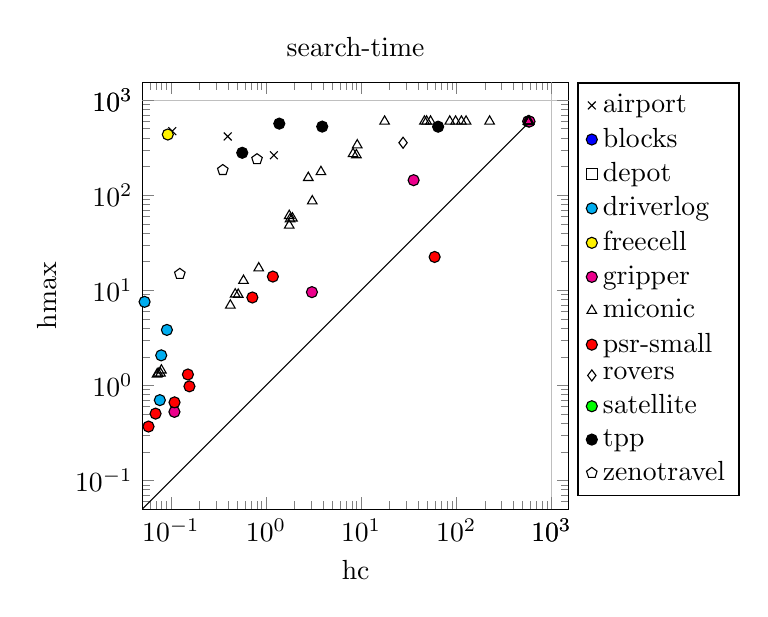
\begin{tikzpicture}
\begin{axis}[extra x tick style={grid=major}, extra x ticks=1000, extra y tick style={grid=major}, extra y ticks=1000, 
height=7.00cm, legend cell align=left, legend style={at={(1.4, 1)}}, title=search-time, width=7.00cm, xlabel=hc, xmin=0.05, xmode=log, ylabel=hmax, ymin=0.05, ymode=log]
\addplot[color=green, mark=x, mark options={{draw=black}}, only marks] coordinates {
(0.010000, 0.016491) (0.016494, 6.755030) (0.010000, 0.717950) (0.010000, 0.590599) (0.395736, 414.959000) (0.103385, 472.065000) (0.010000, 0.010000) (1.210125, 263.493000) (0.010000, 0.015102) (0.010000, 0.016054) (0.010000, 0.015509) (0.010000, 0.687614) (0.010000, 32.734900)
};
\addlegendentry{airport}
\addplot[color=blue, mark=*, mark options={{draw=black}}, only marks] coordinates {
(0.021018, 0.372409) (0.010000, 0.050527) (0.012726, 0.308366) (0.010000, 0.066047) (0.010000, 0.019459) (0.010430, 0.241785) (0.020812, 0.344101) (0.010000, 0.020340) (0.021315, 0.474589) (0.010446, 0.194772) (0.010000, 0.010000) (0.010000, 0.066848) (0.010000, 0.018284)
};
\addlegendentry{blocks}
\addplot[color=magenta, mark=square, mark options={{draw=black}}, only marks] coordinates {
(0.010000, 0.031612) (0.044016, 9.777910) (0.010000, 0.459406) (0.010000, 0.010000) (0.018111, 1.893310) (0.011065, 0.716715)
};
\addlegendentry{depot}
\addplot[color=cyan, mark=*, mark options={{draw=black}}, only marks] coordinates {
(0.079113, 2.071450) (0.011772, 0.146100) (0.010000, 0.010000) (0.010000, 0.038347) (0.012175, 0.432243) (0.090763, 3.835300) (0.042196, 1.016020) (0.076491, 0.700432) (0.022317, 0.523188) (0.052872, 7.568230) (0.029184, 1.031880)
};
\addlegendentry{driverlog}
\addplot[color=yellow, mark=*, mark options={{draw=black}}, only marks] coordinates {
(0.025467, 543.707805) (0.010000, 7.079400) (0.010000, 342.542000) (0.010000, 1.322830) (0.017503, 54.521000) (0.010000, 163.241000) (0.047170, 264.016000) (0.010000, 1.283090) (0.033165, 152.929000) (0.010000, 1.461090) (0.010114, 34.483100) (0.010000, 98.255600) (0.012825, 443.515000) (0.010000, 0.524055) (0.010000, 68.535000) (0.010000, 0.520173) (0.010000, 0.523277) (0.010508, 235.652000) (0.010000, 0.446854) (0.010000, 6.151280) (0.010000, 1.360380) (0.010000, 238.460000) (0.010000, 1.073300) (0.031360, 438.364005) (0.044098, 526.096000) (0.037899, 517.092605) (0.014858, 516.261105) (0.092770, 435.115005) (0.010000, 1.437480) (0.029469, 148.491000) (0.010000, 0.190178) (0.010000, 8.337660) (0.010000, 7.290870) (0.010000, 0.523382) (0.010000, 0.067749) (0.027610, 448.797605) (0.010000, 321.654000) (0.010000, 6.312610) (0.010000, 6.952450) (0.015431, 493.080105) (0.010135, 44.046300) (0.010000, 0.519870) (0.030210, 464.824105)
};
\addlegendentry{freecell}
\addplot[color=magenta, mark=*, mark options={{draw=black}}, only marks] coordinates {
(0.108904, 0.527269) (0.010000, 0.053869) (35.658600, 144.022000) (580.503765, 598.073514) (3.040280, 9.573330) (0.010000, 0.010000) (570.510251, 598.167887) (589.880727, 596.319431)
};
\addlegendentry{gripper}
\addplot[color=cyan, mark=triangle, mark options={{draw=black}}, only marks] coordinates {
(224.446000, 597.933579) (0.510274, 9.035710) (573.474019, 597.365275) (1.788500, 56.040000) (8.228750, 272.530000) (0.579897, 12.645000) (0.021994, 0.305318) (0.010000, 0.013467) (1.897180, 57.236000) (9.107240, 336.694000) (0.073420, 1.336390) (583.477356, 599.408217) (0.474537, 9.099500) (0.010000, 0.054482) (0.010000, 0.020015) (0.010000, 0.019408) (569.532000, 597.087791) (0.079419, 1.444580) (48.852000, 597.974743) (126.919000, 598.062657) (2.784220, 152.824000) (1.754290, 48.142100) (113.458000, 597.760290) (0.010899, 0.074368) (85.522600, 597.865548) (0.010000, 0.019519) (98.525400, 597.754485) (0.019884, 0.260593) (53.705700, 597.862635) (0.010000, 0.010000) (8.918480, 264.814000) (577.266961, 592.260441) (0.011328, 0.066050) (0.010000, 0.052879) (579.359401, 596.516783) (577.410498, 596.063198) (17.665800, 597.651457) (3.781750, 176.252000) (0.838683, 17.129900) (0.011444, 0.070371) (0.010000, 0.019296) (0.071420, 1.306580) (0.077724, 1.337580) (0.019188, 0.208439) (0.421684, 6.954340) (0.034272, 0.414753) (3.065430, 86.787300) (0.041777, 0.485996) (46.340500, 598.207505) (1.755410, 60.925600)
};
\addlegendentry{miconic}
\addplot[color=red, mark=*, mark options={{draw=black}}, only marks] coordinates {
(0.010000, 0.030722) (0.010000, 0.057003) (0.010000, 0.013188) (0.015711, 0.135814) (0.014667, 0.102157) (0.010000, 0.010121) (0.010000, 0.018390) (0.718811, 8.410160) (0.010000, 0.036949) (0.010000, 0.016502) (0.150947, 1.303090) (0.010000, 0.038536) (0.010000, 0.021252) (0.015564, 0.141229) (0.068998, 0.505190) (0.019144, 0.093764) (0.010534, 0.043708) (0.156583, 0.977566) (0.010000, 0.044692) (1.180550, 13.957400) (0.058158, 0.369399) (0.013244, 0.051112) (0.010000, 0.015697) (0.010000, 0.058230) (0.109162, 0.663662) (0.010000, 0.010000) (59.320100, 22.437753)
};
\addlegendentry{psr-small}
\addplot[color=blue, mark=diamond, mark options={{draw=black}}, only marks] coordinates {
(0.019173, 0.293917) (27.633300, 356.412000) (0.044183, 0.495889) (0.010000, 0.010000)
};
\addlegendentry{rovers}
\addplot[color=green, mark=*, mark options={{draw=black}}, only marks] coordinates {
(0.010000, 0.013571) (0.010000, 0.010000) (0.021058, 1.343910) (0.031887, 12.418500) (0.010000, 0.014210) (0.019496, 0.882318)
};
\addlegendentry{satellite}
\addplot[color=black, mark=*, mark options={{draw=black}}, only marks] coordinates {
(3.901330, 526.821972) (0.010000, 0.015316) (0.044292, 10.255400) (0.010000, 0.359451) (1.379290, 566.276805) (0.010000, 0.010000) (0.562574, 279.485000) (64.543100, 525.581644)
};
\addlegendentry{tpp}
\addplot[color=red, mark=pentagon, mark options={{draw=black}}, only marks] coordinates {
(0.014180, 0.211603) (0.032232, 3.192170) (0.010000, 0.020350) (0.010000, 0.012913) (0.010000, 0.027564) (0.804290, 239.404000) (0.124137, 14.887400) (0.010000, 0.010000) (0.351318, 184.058000) (0.010000, 0.077096) (0.010000, 0.016207)
};
\addlegendentry{zenotravel}
\addplot[color=black] coordinates {(0.050000, 0.050000) (599, 599)};
\end{axis}
\end{tikzpicture}
\\
        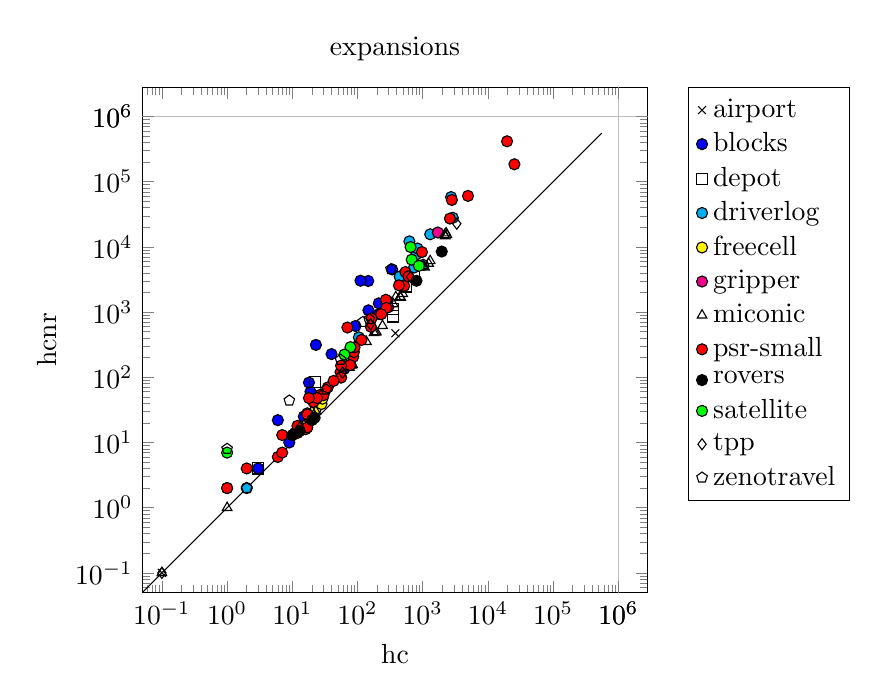
\begin{tikzpicture}
\begin{axis}[extra x tick style={grid=major}, extra x ticks=1000000, extra y tick style={grid=major}, extra y ticks=1000000, 
height=8cm, legend cell align=left, legend style={at={(1.4, 1)}}, title=expansions, width=8.00cm, xlabel=hc, xmin=0.05, xmode=log, ylabel=hcnr, ymin=0.05, ymode=log]
\addplot[color=green, mark=x, mark options={{draw=black}}, only marks] coordinates {
(381, 473) (0.100000, 0.100000) (18, 18)
};
\addlegendentry{airport}
\addplot[color=blue, mark=*, mark options={{draw=black}}, only marks] coordinates {
(1, 2) (40, 227) (147, 1065) (19, 60) (63, 135) (146, 3001) (15, 25) (3, 4) (93, 611) (111, 3029) (340, 4510) (213, 931) (9, 10) (18, 83) (23, 314) (6, 22) (212, 1362) (289, 1470)
};
\addlegendentry{blocks}
\addplot[color=magenta, mark=square, mark options={{draw=black}}, only marks] coordinates {
(22, 84) (347, 858) (352, 1102) (551, 2477) (3, 4) (729, 3670)
};
\addlegendentry{depot}
\addplot[color=cyan, mark=*, mark options={{draw=black}}, only marks] coordinates {
(105, 410) (793, 7645) (835, 9442) (737, 4825) (1304, 15612) (2896, 27945) (1017, 5306) (625, 12152) (2, 2) (2726, 58064) (443, 3510)
};
\addlegendentry{driverlog}
\addplot[color=yellow, mark=*, mark options={{draw=black}}, only marks] coordinates {
(17, 19) (17, 28) (23, 33) (28, 39) (29, 47)
};
\addlegendentry{freecell}
\addplot[color=magenta, mark=*, mark options={{draw=black}}, only marks] coordinates {
(1707, 16634) (296, 1188) (56, 100)
};
\addlegendentry{gripper}
\addplot[color=cyan, mark=triangle, mark options={{draw=black}}, only marks] coordinates {
(20, 25) (1233, 5566) (0.100000, 0.100000) (82, 156) (460, 1675) (137, 351) (449, 1726) (23, 30) (54, 106) (20, 30) (1028, 4987) (84, 156) (1025, 5152) (179, 481) (242, 619) (1, 1) (1302, 6110) (2228, 14732) (187, 488) (493, 1916) (386, 1711) (2159, 15261) (2352, 15271) (195, 495) (22, 25) (1069, 4857) (354, 1334) (80, 153) (2282, 16310) (19, 25) (75, 141)
};
\addlegendentry{miconic}
\addplot[color=red, mark=*, mark options={{draw=black}}, only marks] coordinates {
(19675, 416544) (78, 156) (974, 8330) (160, 597) (115, 374) (6, 6) (272, 1545) (22, 44) (7, 7) (2614, 27214) (277, 1161) (16, 16) (21, 42) (11, 14) (521, 2527) (55, 120) (4955, 60566) (1, 2) (543, 4117) (59, 149) (86, 206) (602, 3537) (27, 54) (88, 244) (70, 580) (12, 14) (30, 53) (18, 24) (24, 48) (77, 154) (12, 18) (56, 151) (17, 27) (35, 70) (231, 928) (18, 48) (90, 288) (7, 13) (2800, 52482) (17, 17) (56, 99) (25480, 185128) (43, 88) (164, 801) (2, 4) (432, 2572)
};
\addlegendentry{psr-small}
\addplot[color=black, mark=*, mark options={{draw=black}}, only marks] coordinates {
(22, 24) (10, 13) (13, 15) (1960, 8490) (803, 3022) (20, 22)
};
\addlegendentry{rovers}
\addplot[color=green, mark=*, mark options={{draw=black}}, only marks] coordinates {
(652, 9941) (678, 6371) (876, 5124) (1, 7) (78, 290) (63, 223)
};
\addlegendentry{satellite}
\addplot[color=blue, mark=diamond, mark options={{draw=black}}, only marks] coordinates {
(3331, 22681) (649, 3465) (158, 648) (13, 17) (0.100000, 0.100000) (59, 118)
};
\addlegendentry{tpp}
\addplot[color=red, mark=pentagon, mark options={{draw=black}}, only marks] coordinates {
(121, 708) (1, 8) (55, 186) (2, 2) (151, 780) (326, 4556) (33, 65) (9, 44)
};
\addlegendentry{zenotravel}
\addplot[color=black] coordinates {(0.050000, 0.050000) (556807, 556807)};
\end{axis}
\end{tikzpicture}
\\
        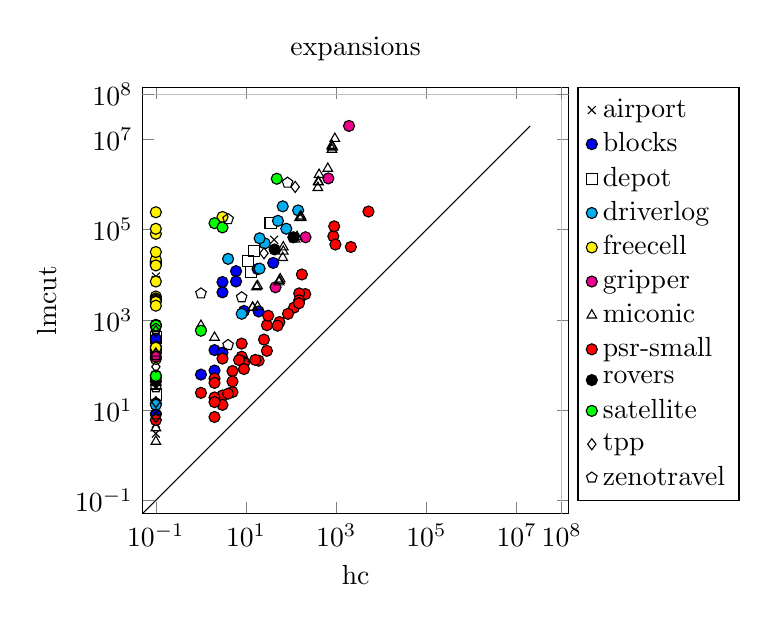
\begin{tikzpicture}
\begin{axis}[extra x tick style={grid=major}, extra x ticks=100000000, extra y tick style={grid=major}, extra y ticks=100000000, 
height=7.00cm, legend cell align=left, legend style={at={(1.4, 1)}}, title=expansions, width=7.00cm, xlabel=hc, xmin=0.05, xmode=log, ylabel=lmcut, ymin=0.05, ymode=log]
\addplot[color=green, mark=x, mark options={{draw=black}}, only marks] coordinates {
(0.100000, 33) (0.100000, 219) (0.100000, 181) (42, 59492) (0.100000, 217) (0.100000, 6) (0.100000, 9131) (0.100000, 5) (0.100000, 7615) (0.100000, 7625) (0.100000, 245) (0.100000, 3) (0.100000, 8)
};
\addlegendentry{airport}
\addplot[color=blue, mark=*, mark options={{draw=black}}, only marks] coordinates {
(18, 13376) (0.100000, 187) (2, 213) (6, 12007) (0.100000, 58) (6, 7076) (9, 1570) (0.100000, 14) (19, 1532) (3, 4066) (2, 75) (0.100000, 379) (3, 6886) (40, 18268) (1, 61) (0.100000, 8) (3, 187)
};
\addlegendentry{blocks}
\addplot[color=magenta, mark=square, mark options={{draw=black}}, only marks] coordinates {
(0.100000, 22) (15, 34039) (11, 20162) (35, 142452) (13, 11292) (0.100000, 407)
};
\addlegendentry{depot}
\addplot[color=cyan, mark=*, mark options={{draw=black}}, only marks] coordinates {
(0.100000, 16896) (26, 49620) (20, 64248) (51, 156560) (0.100000, 13) (143, 266848) (4, 22448) (65, 328115) (20, 13650) (8, 1360) (78, 104720)
};
\addlegendentry{driverlog}
\addplot[color=yellow, mark=*, mark options={{draw=black}}, only marks] coordinates {
(0.100000, 17761) (0.100000, 3286) (0.100000, 2971) (0.100000, 7067) (0.100000, 19591) (0.100000, 242704) (0.100000, 19141) (0.100000, 21631) (0.100000, 226) (0.100000, 136) (0.100000, 211) (0.100000, 2791) (3, 190470) (0.100000, 2626) (0.100000, 256) (0.100000, 16051) (0.100000, 241) (0.100000, 2506) (0.100000, 80809) (0.100000, 2056) (0.100000, 31823) (0.100000, 766) (0.100000, 104311)
};
\addlegendentry{freecell}
\addplot[color=magenta, mark=*, mark options={{draw=black}}, only marks] coordinates {
(1920, 19916814) (45, 5268) (208, 67710) (0.100000, 151) (668, 1367176)
};
\addlegendentry{gripper}
\addplot[color=cyan, mark=triangle, mark options={{draw=black}}, only marks] coordinates {
(55, 7443) (0.100000, 181) (135, 69039) (155, 185047) (18, 5647) (819, 6915236) (156, 182083) (0.100000, 43) (2, 406) (395, 1143604) (409, 1131564) (17, 5356) (824, 6718966) (803, 5972930) (54, 6872) (18, 1954) (14, 1892) (416, 1656749) (0.100000, 50) (67, 40958) (0.100000, 4) (122, 60879) (57, 8012) (65, 23797) (166, 185293) (391, 846923) (931, 10411953) (649, 2261005) (14, 1861) (801, 7337121) (164, 198138) (1, 745) (0.100000, 2) (67, 32915)
};
\addlegendentry{miconic}
\addplot[color=red, mark=*, mark options={{draw=black}}, only marks] coordinates {
(5, 73) (206, 3719) (863, 71216) (902, 118208) (3, 21) (29, 760) (8, 152) (19, 124) (958, 46688) (9, 116) (116, 1866) (55, 892) (151, 3851) (3, 138) (31, 1232) (25, 364) (8, 297) (5, 25) (4, 23) (0.100000, 772) (9, 109) (173, 10124) (3, 13) (2109, 41214) (29, 205) (5183, 251714) (85, 1355) (1, 24) (2, 19) (2, 7) (151, 2707) (7, 128) (2, 50) (2, 40) (5, 43) (16, 129) (0.100000, 6) (9, 81) (2, 15) (50, 741) (149, 2328)
};
\addlegendentry{psr-small}
\addplot[color=black, mark=*, mark options={{draw=black}}, only marks] coordinates {
(43, 36383) (0.100000, 43) (0.100000, 50) (112, 67588)
};
\addlegendentry{rovers}
\addplot[color=green, mark=*, mark options={{draw=black}}, only marks] coordinates {
(0.100000, 57) (2, 138858) (48, 1342395) (0.100000, 745) (1, 573) (3, 112017)
};
\addlegendentry{satellite}
\addplot[color=blue, mark=diamond, mark options={{draw=black}}, only marks] coordinates {
(0.100000, 91) (0.100000, 15) (0.100000, 559) (0.100000, 7) (25, 29953) (123, 884427)
};
\addlegendentry{tpp}
\addplot[color=red, mark=pentagon, mark options={{draw=black}}, only marks] coordinates {
(0.100000, 8) (0.100000, 632) (1, 3844) (0.100000, 166) (4, 170892) (8, 3160) (83, 1096013) (0.100000, 32) (4, 276)
};
\addlegendentry{zenotravel}
\addplot[color=black] coordinates {(0.050000, 0.050000) (19916814, 19916814)};
\end{axis}
\end{tikzpicture}
\\
        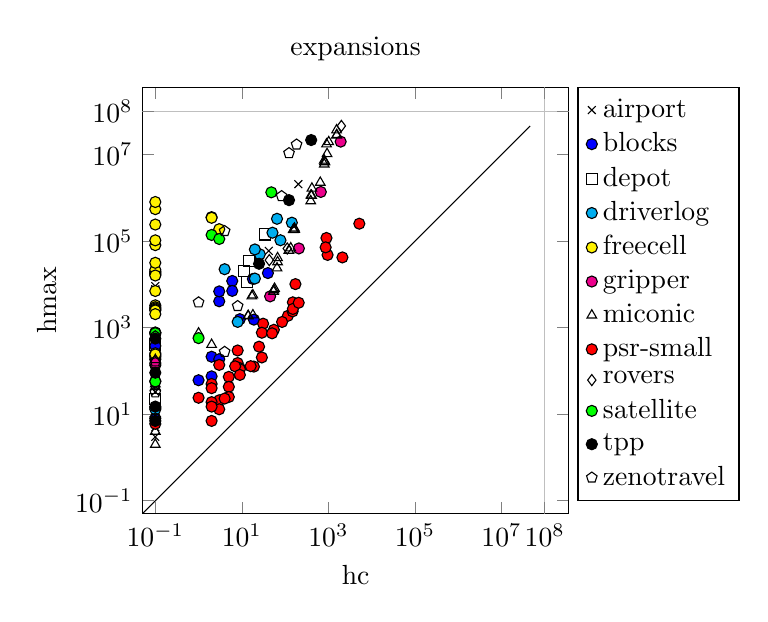
\begin{tikzpicture}
\begin{axis}[extra x tick style={grid=major}, extra x ticks=100000000, extra y tick style={grid=major}, extra y ticks=100000000, 
height=7.00cm, legend cell align=left, legend style={at={(1.4, 1)}}, title=expansions, width=7.00cm, xlabel=hc, xmin=0.05, xmode=log, ylabel=hmax, ymin=0.05, ymode=log]
\addplot[color=green, mark=x, mark options={{draw=black}}, only marks] coordinates {
(42, 59583) (0.100000, 33) (0.100000, 219) (0.100000, 181) (0.100000, 6) (0.100000, 217) (0.100000, 245) (202, 2073240) (0.100000, 9131) (0.100000, 5) (0.100000, 7615) (0.100000, 7625) (0.100000, 3) (0.100000, 8)
};
\addlegendentry{airport}
\addplot[color=blue, mark=*, mark options={{draw=black}}, only marks] coordinates {
(9, 1572) (18, 13376) (0.100000, 379) (6, 12007) (0.100000, 58) (6, 7076) (0.100000, 14) (2, 213) (3, 4066) (2, 75) (0.100000, 187) (40, 18270) (3, 6886) (1, 61) (0.100000, 8) (3, 187) (19, 1534)
};
\addlegendentry{blocks}
\addplot[color=magenta, mark=square, mark options={{draw=black}}, only marks] coordinates {
(0.100000, 22) (35, 142466) (13, 11292) (11, 20161) (15, 34032) (0.100000, 407)
};
\addlegendentry{depot}
\addplot[color=cyan, mark=*, mark options={{draw=black}}, only marks] coordinates {
(0.100000, 16896) (26, 49620) (20, 64248) (51, 156560) (0.100000, 13) (143, 266816) (4, 22448) (20, 13650) (8, 1360) (65, 328078) (78, 104720)
};
\addlegendentry{driverlog}
\addplot[color=yellow, mark=*, mark options={{draw=black}}, only marks] coordinates {
(0.100000, 17761) (0.100000, 3286) (0.100000, 2971) (0.100000, 19591) (2, 357856) (0.100000, 19141) (0.100000, 548746) (0.100000, 21631) (0.100000, 226) (0.100000, 136) (0.100000, 802036) (0.100000, 211) (0.100000, 2791) (0.100000, 31561) (0.100000, 2626) (0.100000, 7036) (0.100000, 256) (0.100000, 16051) (0.100000, 241) (0.100000, 80806) (0.100000, 2506) (0.100000, 2056) (2, 346276) (3, 188791) (0.100000, 766) (0.100000, 104311) (0.100000, 241546)
};
\addlegendentry{freecell}
\addplot[color=magenta, mark=*, mark options={{draw=black}}, only marks] coordinates {
(1920, 19918398) (668, 1368076) (208, 67738) (0.100000, 151) (45, 5283)
};
\addlegendentry{gripper}
\addplot[color=cyan, mark=triangle, mark options={{draw=black}}, only marks] coordinates {
(395, 1143601) (0.100000, 181) (18, 5647) (409, 1131640) (0.100000, 43) (801, 7341225) (17, 5356) (1563, 28711853) (67, 40955) (391, 846921) (931, 10420707) (18, 1954) (803, 5975018) (55, 7441) (0.100000, 50) (907, 17460317) (122, 60875) (1019, 19611126) (156, 182080) (166, 185292) (819, 6917972) (155, 185045) (1542, 36749162) (65, 23798) (54, 6870) (824, 6722843) (0.100000, 4) (1545, 27889713) (649, 2261740) (14, 1861) (416, 1656947) (67, 32916) (57, 8012) (2, 406) (1, 745) (14, 1892) (164, 198133) (135, 69035) (0.100000, 2)
};
\addlegendentry{miconic}
\addplot[color=red, mark=*, mark options={{draw=black}}, only marks] coordinates {
(116, 1880) (5, 73) (902, 118208) (3, 21) (173, 10156) (8, 152) (2, 19) (9, 116) (5, 43) (55, 892) (151, 3851) (3, 138) (25, 364) (8, 297) (5, 25) (4, 23) (149, 2378) (5183, 252962) (0.100000, 772) (31, 1236) (958, 47992) (9, 109) (1, 24) (3, 13) (29, 764) (2109, 42030) (29, 205) (85, 1355) (19, 126) (2, 7) (151, 2707) (7, 128) (2, 50) (863, 71716) (2, 40) (16, 129) (0.100000, 6) (206, 3759) (9, 81) (2, 15) (50, 741)
};
\addlegendentry{psr-small}
\addplot[color=blue, mark=diamond, mark options={{draw=black}}, only marks] coordinates {
(0.100000, 43) (112, 67588) (43, 36387) (1997, 45935775) (0.100000, 50)
};
\addlegendentry{rovers}
\addplot[color=green, mark=*, mark options={{draw=black}}, only marks] coordinates {
(0.100000, 57) (48, 1342391) (2, 138858) (0.100000, 745) (1, 573) (3, 112017)
};
\addlegendentry{satellite}
\addplot[color=black, mark=*, mark options={{draw=black}}, only marks] coordinates {
(0.100000, 91) (0.100000, 559) (0.100000, 15) (400, 21653693) (0.100000, 7) (123, 884552) (25, 29955)
};
\addlegendentry{tpp}
\addplot[color=red, mark=pentagon, mark options={{draw=black}}, only marks] coordinates {
(0.100000, 8) (123, 10801620) (83, 1096038) (8, 3160) (0.100000, 632) (1, 3844) (0.100000, 166) (4, 170892) (0.100000, 32) (4, 276) (184, 17075893)
};
\addlegendentry{zenotravel}
\addplot[color=black] coordinates {(0.050000, 0.050000) (45935775, 45935775)};
\end{axis}
\end{tikzpicture}

    \end{center}


    \subsubsection*{Cost Bound 0.75}

    \begin{center}

        \begin{tabular}{l|r|r|r|r}
            Finished PPD1 & hc & hcnr & hmax & lmcut \\\hline
            airport (19) & 8 & 8 & \textbf{16} & 15\\\hline
            blocks (18) & \textbf{18} & \textbf{18} & 15 & 15 \\\hline
            depot (6) & 3 & 3 & \textbf{4} & 2 \\\hline
            driverlog (11) & \textbf{9} & \textbf{9} & 6 & 3 \\\hline
            freecell (55) & 0 & 0 & \textbf{13} & 7 \\\hline
            gripper (8) & 3 & 3 & \textbf{4} & \textbf{4} \\\hline
            miconic (69) & 35 & \textbf{39} & \textbf{39} & \textbf{39} \\\hline
            PSR (49) & \textbf{47} & 45 & 46 & 46 \\\hline
            rovers (7) & 4 & 5 & \textbf{6} & 4 \\\hline
            satellite (6) & 4 & \textbf{5} & 4 & 4 \\\hline
            tpp (10) & 4 & \textbf{5} & \textbf{5} & 4 \\\hline
            zenotravel (11) & \textbf{8} & \textbf{8} & 7 & 6 \\\hline\hline
            sum (269) & 143 & 148 & \textbf{165} & 149 \\
        \end{tabular}

        \scriptsize
        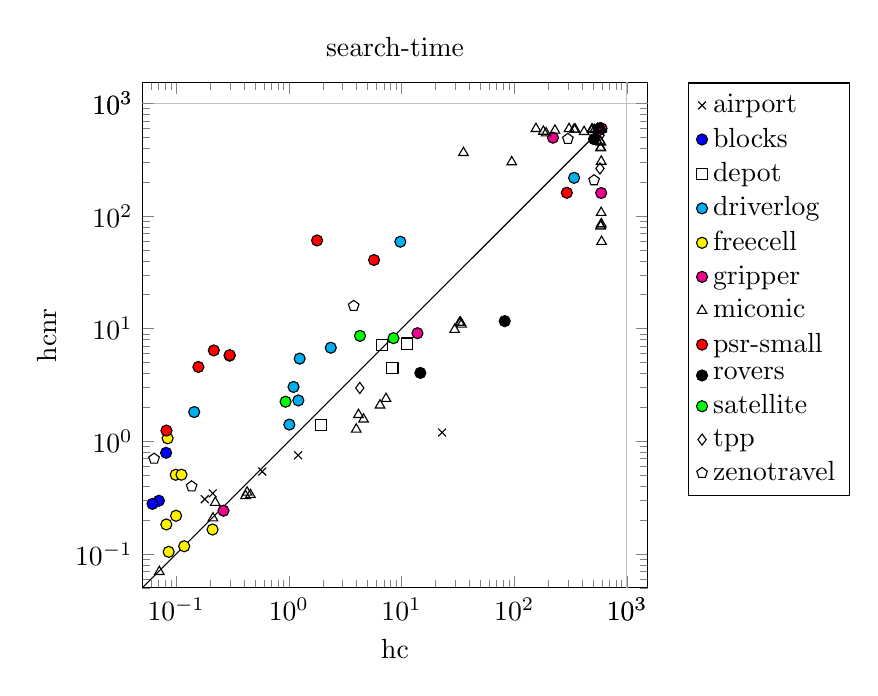
\begin{tikzpicture}
\begin{axis}[extra x tick style={grid=major}, extra x ticks=1000, extra y tick style={grid=major}, 
extra y ticks=1000, height=8cm, legend cell align=left, legend style={at={(1.4, 1)}}, title=search-time, width=8cm, xlabel=hc, xmin=0.05, xmode=log, ylabel=hcnr, ymin=0.05, ymode=log]
\addplot[color=green, mark=x, mark options={{draw=black}}, only marks] coordinates {
(0.580962, 0.539156) (22.919350, 1.197450) (1.207802, 0.751533) (0.010000, 0.010000) (0.211029, 0.344864) (0.179368, 0.306256)
};
\addlegendentry{airport}
\addplot[color=blue, mark=*, mark options={{draw=black}}, only marks] coordinates {
(0.070254, 0.296864) (0.031537, 0.132323) (0.061611, 0.278351) (0.010000, 0.015546) (0.081349, 0.790786) (0.032068, 0.459737) (0.010000, 0.022621) (0.038953, 0.506324) (0.024986, 0.185765) (0.010000, 0.019080) (0.010000, 0.010000) (0.010000, 0.045402) (0.011799, 0.083719)
};
\addlegendentry{blocks}
\addplot[color=magenta, mark=square, mark options={{draw=black}}, only marks] coordinates {
(11.217900, 7.372310) (0.010000, 0.032782) (6.757340, 7.158310) (0.010000, 0.010000) (8.306120, 4.493250) (1.943620, 1.390270)
};
\addlegendentry{depot}
\addplot[color=cyan, mark=*, mark options={{draw=black}}, only marks] coordinates {
(0.297981, 5.756450) (0.144535, 1.819230) (1.100020, 3.040280) (1.214180, 2.305950) (340.116000, 218.241000) (9.760760, 59.133700) (1.246790, 5.421790) (1.009640, 1.408210) (0.013146, 0.044778) (0.010000, 0.010000) (2.354820, 6.773570)
};
\addlegendentry{driverlog}
\addplot[color=yellow, mark=*, mark options={{draw=black}}, only marks] coordinates {
(0.099746, 0.218327) (0.210252, 0.164829) (0.042857, 0.142258) (0.013246, 0.016653) (0.117766, 0.117104) (0.099051, 0.504578) (0.083962, 1.063150) (0.010000, 0.023282) (0.037383, 0.106107) (0.141554, 0.013294) (0.081759, 0.182805) (0.111385, 0.505483) (0.025328, 0.024882) (0.085739, 0.104453)
};
\addlegendentry{freecell}
\addplot[color=magenta, mark=*, mark options={{draw=black}}, only marks] coordinates {
(0.262926, 0.241988) (220.812500, 495.988300) (596.647608, 597.565062) (569.492855, 580.212440) (0.010000, 0.010000) (13.844100, 9.110310) (591.089502, 160.080000)
};
\addlegendentry{gripper}
\addplot[color=cyan, mark=triangle, mark options={{draw=black}}, only marks] coordinates {
(339.622700, 588.378030) (0.010000, 0.011511) (549.845320, 596.864944) (590.112556, 597.189862) (7.282070, 2.391340) (0.010000, 0.012300) (0.412567, 0.327916) (584.148657, 401.133000) (6.442820, 2.091980) (0.039212, 0.046379) (3.963360, 1.277520) (590.819602, 107.059000) (586.187417, 597.268517) (306.656100, 594.349870) (95.053000, 301.677300) (34.077400, 10.919400) (181.635500, 562.785100) (0.010000, 0.012302) (35.450700, 364.431800) (594.301000, 589.966394) (592.930220, 85.041900) (585.482311, 81.044100) (0.026386, 0.042528) (570.608013, 597.167369) (347.818020, 587.793298) (155.906400, 595.750950) (32.738500, 11.323200) (596.722586, 598.978263) (0.070847, 0.069548) (191.937600, 544.281070) (577.370218, 460.882000) (496.366840, 586.208798) (0.042445, 0.049317) (592.167179, 305.104556) (0.455739, 0.335505) (29.592500, 9.804140) (0.048676, 0.049344) (4.148850, 1.722520) (585.890390, 82.624400) (0.212131, 0.208158) (586.905028, 407.188000) (577.634284, 595.238650) (588.228783, 451.849000) (517.980280, 582.901515) (0.222096, 0.285741) (488.742600, 588.815017) (596.108119, 59.254000) (229.859700, 575.452420) (4.599160, 1.569080) (0.010000, 0.010000) (33.443600, 11.359900) (0.425846, 0.352192) (417.259400, 559.410200) (0.010000, 0.012175)
};
\addlegendentry{miconic}
\addplot[color=red, mark=*, mark options={{draw=black}}, only marks] coordinates {
(0.010000, 0.011470) (0.010000, 0.032399) (293.244000, 160.887713) (0.010000, 0.012510) (0.020875, 0.200436) (0.215694, 6.411470) (0.010000, 0.019380) (0.081920, 1.245030) (0.013860, 0.108072) (0.034962, 0.448613) (0.020044, 0.175404) (0.157385, 4.569860) (0.010000, 0.044764) (0.011576, 0.024512) (0.298527, 5.820420) (0.010000, 0.010334) (0.010000, 0.058066) (1.779940, 60.661200) (0.010000, 0.020175) (0.030218, 0.282279) (0.014752, 0.078198) (0.010000, 0.010393) (0.010000, 0.031036) (0.010850, 0.076801) (0.010000, 0.015075) (0.016773, 0.031202) (0.022007, 0.111476) (0.010000, 0.010273) (0.010000, 0.010000) (5.700890, 40.694000)
};
\addlegendentry{psr-small}
\addplot[color=black, mark=*, mark options={{draw=black}}, only marks] coordinates {
(14.684900, 4.047890) (82.362900, 11.664700) (511.206762, 481.269259) (0.010000, 0.010000)
};
\addlegendentry{rovers}
\addplot[color=green, mark=*, mark options={{draw=black}}, only marks] coordinates {
(8.485640, 8.230840) (0.016291, 0.046241) (0.935294, 2.246410) (0.010000, 0.010000) (0.010000, 0.027242) (4.278860, 8.627940)
};
\addlegendentry{satellite}
\addplot[color=blue, mark=diamond, mark options={{draw=black}}, only marks] coordinates {
(578.425608, 519.404647) (4.261390, 2.976200) (0.033617, 0.096048) (576.817000, 264.094000) (0.010000, 0.010000)
};
\addlegendentry{tpp}
\addplot[color=red, mark=pentagon, mark options={{draw=black}}, only marks] coordinates {
(511.621367, 207.755000) (0.018711, 0.085917) (553.269035, 596.441548) (0.010000, 0.020608) (0.063638, 0.701225) (3.762470, 15.939800) (0.010000, 0.010000) (0.010000, 0.016045) (0.010000, 0.011999) (0.137054, 0.398511) (299.509103, 483.854610)
};
\addlegendentry{zenotravel}
\addplot[color=black] coordinates {(0.050000, 0.050000) (598, 598)};
\end{axis}
\end{tikzpicture}
\\
        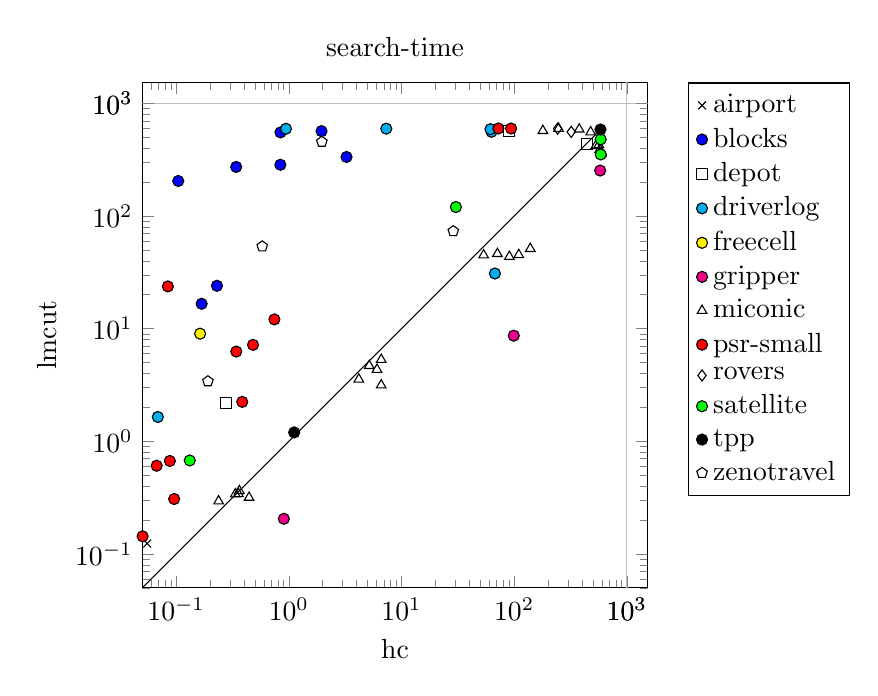
\begin{tikzpicture}
\begin{axis}[extra x tick style={grid=major}, extra x ticks=1000, extra y tick style={grid=major}, extra y ticks=1000, 
height=8.00cm, legend cell align=left, legend style={at={(1.4, 1)}}, title=search-time, width=8.00cm, xlabel=hc, xmin=0.05, xmode=log, ylabel=lmcut, ymin=0.05, ymode=log]
\addplot[color=green, mark=x, mark options={{draw=black}}, only marks] coordinates {
(0.048574, 0.120299) (0.046050, 0.111071) (0.055281, 0.123871) (0.010000, 0.010000) (0.041357, 0.108940)
};
\addlegendentry{airport}
\addplot[color=blue, mark=*, mark options={{draw=black}}, only marks] coordinates {
(0.230047, 24.030000) (0.010000, 0.031479) (0.025873, 4.558310) (0.843013, 552.542811) (0.168246, 16.629000) (0.010000, 0.027709) (0.340901, 272.692000) (1.950830, 566.580613) (3.251590, 334.247000) (0.010000, 0.362648) (0.013312, 0.390551) (0.010000, 0.062532) (0.010000, 0.010000) (0.104296, 204.640000) (0.841473, 285.099000) (0.010000, 0.228853)
};
\addlegendentry{blocks}
\addplot[color=magenta, mark=square, mark options={{draw=black}}, only marks] coordinates {
(0.278061, 2.194290) (0.010000, 0.011175) (441.957403, 437.746983) (90.623300, 571.810165)
};
\addlegendentry{depot}
\addplot[color=cyan, mark=*, mark options={{draw=black}}, only marks] coordinates {
(7.332420, 596.147586) (0.942436, 595.142993) (62.976600, 559.171837) (67.492700, 30.890800) (0.068716, 1.645040) (0.010000, 0.014424) (61.657100, 590.020191)
};
\addlegendentry{driverlog}
\addplot[color=yellow, mark=*, mark options={{draw=black}}, only marks] coordinates {
(0.163048, 9.025770)
};
\addlegendentry{freecell}
\addplot[color=magenta, mark=*, mark options={{draw=black}}, only marks] coordinates {
(0.903325, 0.205256) (580.451050, 253.325000) (0.022548, 0.015056) (99.204100, 8.665220)
};
\addlegendentry{gripper}
\addplot[color=cyan, mark=triangle, mark options={{draw=black}}, only marks] coordinates {
(576.011881, 389.226000) (71.049900, 46.231500) (564.582662, 428.204000) (0.356830, 0.341769) (477.705820, 556.250166) (53.585600, 45.017000) (90.713600, 43.600100) (0.057181, 0.048574) (179.939100, 572.062491) (139.131000, 51.293500) (0.026238, 0.041037) (0.050551, 0.046426) (0.046988, 0.047282) (593.599832, 359.371000) (0.334975, 0.339808) (247.974400, 597.565185) (6.607240, 3.151880) (0.023070, 0.038922) (0.363855, 0.363542) (0.237966, 0.294433) (109.895000, 45.257500) (6.610370, 5.314100) (378.202100, 588.854652) (0.443423, 0.316996) (6.064860, 4.336280) (5.174240, 4.686660) (4.182060, 3.551270) (531.653339, 420.967000) (0.010000, 0.010000)
};
\addlegendentry{miconic}
\addplot[color=red, mark=*, mark options={{draw=black}}, only marks] coordinates {
(0.084348, 23.722300) (93.962700, 598.190931) (0.025299, 0.938619) (0.341576, 6.263790) (0.028221, 26.004900) (0.010000, 0.048287) (0.087873, 0.668967) (0.385828, 2.239800) (0.010000, 0.021130) (0.012386, 0.062160) (0.010000, 0.011759) (0.480840, 7.183010) (0.022369, 0.994706) (0.744401, 12.090800) (0.010000, 0.012970) (0.010000, 0.020451) (0.039768, 0.225446) (0.017934, 0.042342) (0.010000, 0.010892) (0.027529, 0.049036) (72.487900, 599.024594) (0.010000, 0.017533) (0.010000, 0.025226) (0.031668, 0.130135) (0.010000, 0.021697) (0.010000, 0.014396) (0.023448, 0.093158) (0.095937, 0.307649) (0.019262, 0.219040) (0.058920, 0.030411) (0.067107, 0.607171) (0.013632, 0.866814) (0.015867, 0.823189) (0.050345, 0.143485) (0.010000, 0.010000)
};
\addlegendentry{psr-small}
\addplot[color=blue, mark=diamond, mark options={{draw=black}}, only marks] coordinates {
(243.087041, 596.896720) (0.010000, 0.018420) (321.248641, 558.373378) (0.010000, 0.031314) (0.010000, 0.010000) (0.010000, 0.017019)
};
\addlegendentry{rovers}
\addplot[color=green, mark=*, mark options={{draw=black}}, only marks] coordinates {
(30.415200, 120.126000) (0.131941, 0.676322) (0.026147, 0.120091) (586.529861, 479.144000) (587.444295, 351.926000) (0.010000, 0.010000)
};
\addlegendentry{satellite}
\addplot[color=black, mark=*, mark options={{draw=black}}, only marks] coordinates {
(0.018018, 0.022904) (1.115150, 1.199440) (583.635883, 586.030800) (0.010000, 0.010000)
};
\addlegendentry{tpp}
\addplot[color=red, mark=pentagon, mark options={{draw=black}}, only marks] coordinates {
(0.580617, 53.775400) (28.824500, 73.376400) (1.963960, 455.922727) (0.010000, 0.256246) (0.010000, 0.010000) (0.191202, 3.411590) (0.010000, 0.466716)
};
\addlegendentry{zenotravel}
\addplot[color=black] coordinates {(0.050000, 0.050000) (599, 599)};
\end{axis}
\end{tikzpicture}
\\
        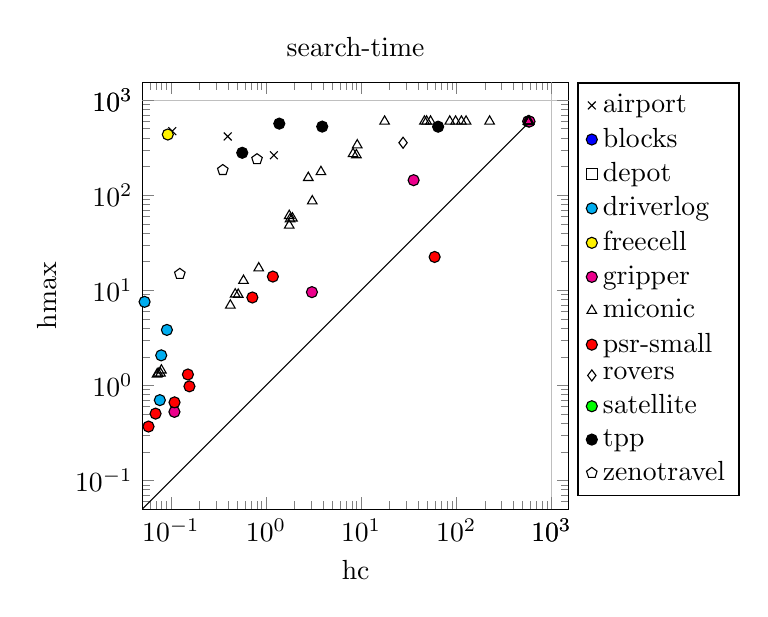
\begin{tikzpicture}
\begin{axis}[extra x tick style={grid=major}, extra x ticks=1000, extra y tick style={grid=major}, extra y ticks=1000, 
height=7.00cm, legend cell align=left, legend style={at={(1.4, 1)}}, title=search-time, width=7.00cm, xlabel=hc, xmin=0.05, xmode=log, ylabel=hmax, ymin=0.05, ymode=log]
\addplot[color=green, mark=x, mark options={{draw=black}}, only marks] coordinates {
(0.010000, 0.016491) (0.016494, 6.755030) (0.010000, 0.717950) (0.010000, 0.590599) (0.395736, 414.959000) (0.103385, 472.065000) (0.010000, 0.010000) (1.210125, 263.493000) (0.010000, 0.015102) (0.010000, 0.016054) (0.010000, 0.015509) (0.010000, 0.687614) (0.010000, 32.734900)
};
\addlegendentry{airport}
\addplot[color=blue, mark=*, mark options={{draw=black}}, only marks] coordinates {
(0.021018, 0.372409) (0.010000, 0.050527) (0.012726, 0.308366) (0.010000, 0.066047) (0.010000, 0.019459) (0.010430, 0.241785) (0.020812, 0.344101) (0.010000, 0.020340) (0.021315, 0.474589) (0.010446, 0.194772) (0.010000, 0.010000) (0.010000, 0.066848) (0.010000, 0.018284)
};
\addlegendentry{blocks}
\addplot[color=magenta, mark=square, mark options={{draw=black}}, only marks] coordinates {
(0.010000, 0.031612) (0.044016, 9.777910) (0.010000, 0.459406) (0.010000, 0.010000) (0.018111, 1.893310) (0.011065, 0.716715)
};
\addlegendentry{depot}
\addplot[color=cyan, mark=*, mark options={{draw=black}}, only marks] coordinates {
(0.079113, 2.071450) (0.011772, 0.146100) (0.010000, 0.010000) (0.010000, 0.038347) (0.012175, 0.432243) (0.090763, 3.835300) (0.042196, 1.016020) (0.076491, 0.700432) (0.022317, 0.523188) (0.052872, 7.568230) (0.029184, 1.031880)
};
\addlegendentry{driverlog}
\addplot[color=yellow, mark=*, mark options={{draw=black}}, only marks] coordinates {
(0.025467, 543.707805) (0.010000, 7.079400) (0.010000, 342.542000) (0.010000, 1.322830) (0.017503, 54.521000) (0.010000, 163.241000) (0.047170, 264.016000) (0.010000, 1.283090) (0.033165, 152.929000) (0.010000, 1.461090) (0.010114, 34.483100) (0.010000, 98.255600) (0.012825, 443.515000) (0.010000, 0.524055) (0.010000, 68.535000) (0.010000, 0.520173) (0.010000, 0.523277) (0.010508, 235.652000) (0.010000, 0.446854) (0.010000, 6.151280) (0.010000, 1.360380) (0.010000, 238.460000) (0.010000, 1.073300) (0.031360, 438.364005) (0.044098, 526.096000) (0.037899, 517.092605) (0.014858, 516.261105) (0.092770, 435.115005) (0.010000, 1.437480) (0.029469, 148.491000) (0.010000, 0.190178) (0.010000, 8.337660) (0.010000, 7.290870) (0.010000, 0.523382) (0.010000, 0.067749) (0.027610, 448.797605) (0.010000, 321.654000) (0.010000, 6.312610) (0.010000, 6.952450) (0.015431, 493.080105) (0.010135, 44.046300) (0.010000, 0.519870) (0.030210, 464.824105)
};
\addlegendentry{freecell}
\addplot[color=magenta, mark=*, mark options={{draw=black}}, only marks] coordinates {
(0.108904, 0.527269) (0.010000, 0.053869) (35.658600, 144.022000) (580.503765, 598.073514) (3.040280, 9.573330) (0.010000, 0.010000) (570.510251, 598.167887) (589.880727, 596.319431)
};
\addlegendentry{gripper}
\addplot[color=cyan, mark=triangle, mark options={{draw=black}}, only marks] coordinates {
(224.446000, 597.933579) (0.510274, 9.035710) (573.474019, 597.365275) (1.788500, 56.040000) (8.228750, 272.530000) (0.579897, 12.645000) (0.021994, 0.305318) (0.010000, 0.013467) (1.897180, 57.236000) (9.107240, 336.694000) (0.073420, 1.336390) (583.477356, 599.408217) (0.474537, 9.099500) (0.010000, 0.054482) (0.010000, 0.020015) (0.010000, 0.019408) (569.532000, 597.087791) (0.079419, 1.444580) (48.852000, 597.974743) (126.919000, 598.062657) (2.784220, 152.824000) (1.754290, 48.142100) (113.458000, 597.760290) (0.010899, 0.074368) (85.522600, 597.865548) (0.010000, 0.019519) (98.525400, 597.754485) (0.019884, 0.260593) (53.705700, 597.862635) (0.010000, 0.010000) (8.918480, 264.814000) (577.266961, 592.260441) (0.011328, 0.066050) (0.010000, 0.052879) (579.359401, 596.516783) (577.410498, 596.063198) (17.665800, 597.651457) (3.781750, 176.252000) (0.838683, 17.129900) (0.011444, 0.070371) (0.010000, 0.019296) (0.071420, 1.306580) (0.077724, 1.337580) (0.019188, 0.208439) (0.421684, 6.954340) (0.034272, 0.414753) (3.065430, 86.787300) (0.041777, 0.485996) (46.340500, 598.207505) (1.755410, 60.925600)
};
\addlegendentry{miconic}
\addplot[color=red, mark=*, mark options={{draw=black}}, only marks] coordinates {
(0.010000, 0.030722) (0.010000, 0.057003) (0.010000, 0.013188) (0.015711, 0.135814) (0.014667, 0.102157) (0.010000, 0.010121) (0.010000, 0.018390) (0.718811, 8.410160) (0.010000, 0.036949) (0.010000, 0.016502) (0.150947, 1.303090) (0.010000, 0.038536) (0.010000, 0.021252) (0.015564, 0.141229) (0.068998, 0.505190) (0.019144, 0.093764) (0.010534, 0.043708) (0.156583, 0.977566) (0.010000, 0.044692) (1.180550, 13.957400) (0.058158, 0.369399) (0.013244, 0.051112) (0.010000, 0.015697) (0.010000, 0.058230) (0.109162, 0.663662) (0.010000, 0.010000) (59.320100, 22.437753)
};
\addlegendentry{psr-small}
\addplot[color=blue, mark=diamond, mark options={{draw=black}}, only marks] coordinates {
(0.019173, 0.293917) (27.633300, 356.412000) (0.044183, 0.495889) (0.010000, 0.010000)
};
\addlegendentry{rovers}
\addplot[color=green, mark=*, mark options={{draw=black}}, only marks] coordinates {
(0.010000, 0.013571) (0.010000, 0.010000) (0.021058, 1.343910) (0.031887, 12.418500) (0.010000, 0.014210) (0.019496, 0.882318)
};
\addlegendentry{satellite}
\addplot[color=black, mark=*, mark options={{draw=black}}, only marks] coordinates {
(3.901330, 526.821972) (0.010000, 0.015316) (0.044292, 10.255400) (0.010000, 0.359451) (1.379290, 566.276805) (0.010000, 0.010000) (0.562574, 279.485000) (64.543100, 525.581644)
};
\addlegendentry{tpp}
\addplot[color=red, mark=pentagon, mark options={{draw=black}}, only marks] coordinates {
(0.014180, 0.211603) (0.032232, 3.192170) (0.010000, 0.020350) (0.010000, 0.012913) (0.010000, 0.027564) (0.804290, 239.404000) (0.124137, 14.887400) (0.010000, 0.010000) (0.351318, 184.058000) (0.010000, 0.077096) (0.010000, 0.016207)
};
\addlegendentry{zenotravel}
\addplot[color=black] coordinates {(0.050000, 0.050000) (599, 599)};
\end{axis}
\end{tikzpicture}
\\
        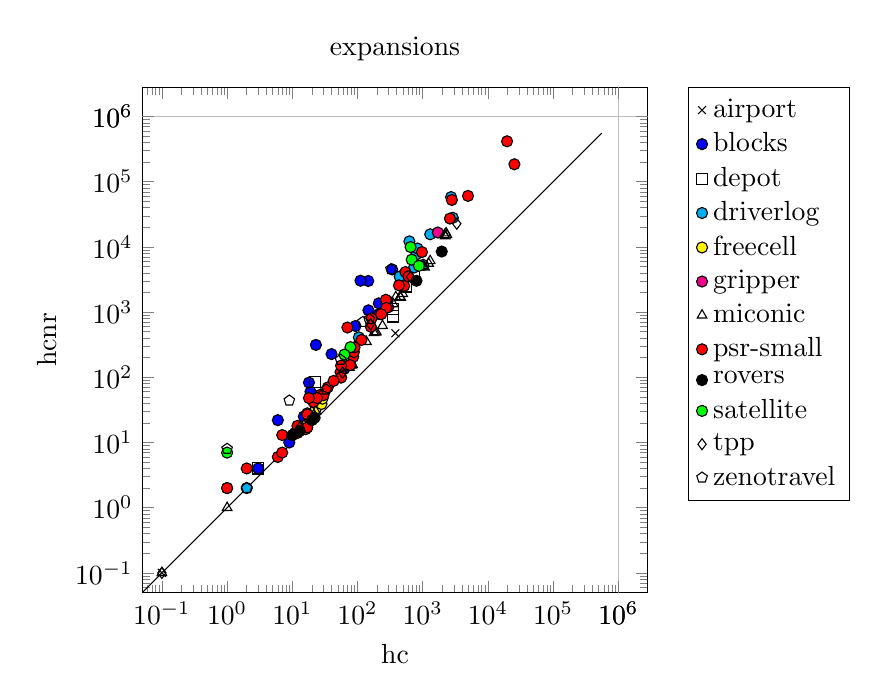
\begin{tikzpicture}
\begin{axis}[extra x tick style={grid=major}, extra x ticks=1000000, extra y tick style={grid=major}, extra y ticks=1000000, 
height=8cm, legend cell align=left, legend style={at={(1.4, 1)}}, title=expansions, width=8.00cm, xlabel=hc, xmin=0.05, xmode=log, ylabel=hcnr, ymin=0.05, ymode=log]
\addplot[color=green, mark=x, mark options={{draw=black}}, only marks] coordinates {
(381, 473) (0.100000, 0.100000) (18, 18)
};
\addlegendentry{airport}
\addplot[color=blue, mark=*, mark options={{draw=black}}, only marks] coordinates {
(1, 2) (40, 227) (147, 1065) (19, 60) (63, 135) (146, 3001) (15, 25) (3, 4) (93, 611) (111, 3029) (340, 4510) (213, 931) (9, 10) (18, 83) (23, 314) (6, 22) (212, 1362) (289, 1470)
};
\addlegendentry{blocks}
\addplot[color=magenta, mark=square, mark options={{draw=black}}, only marks] coordinates {
(22, 84) (347, 858) (352, 1102) (551, 2477) (3, 4) (729, 3670)
};
\addlegendentry{depot}
\addplot[color=cyan, mark=*, mark options={{draw=black}}, only marks] coordinates {
(105, 410) (793, 7645) (835, 9442) (737, 4825) (1304, 15612) (2896, 27945) (1017, 5306) (625, 12152) (2, 2) (2726, 58064) (443, 3510)
};
\addlegendentry{driverlog}
\addplot[color=yellow, mark=*, mark options={{draw=black}}, only marks] coordinates {
(17, 19) (17, 28) (23, 33) (28, 39) (29, 47)
};
\addlegendentry{freecell}
\addplot[color=magenta, mark=*, mark options={{draw=black}}, only marks] coordinates {
(1707, 16634) (296, 1188) (56, 100)
};
\addlegendentry{gripper}
\addplot[color=cyan, mark=triangle, mark options={{draw=black}}, only marks] coordinates {
(20, 25) (1233, 5566) (0.100000, 0.100000) (82, 156) (460, 1675) (137, 351) (449, 1726) (23, 30) (54, 106) (20, 30) (1028, 4987) (84, 156) (1025, 5152) (179, 481) (242, 619) (1, 1) (1302, 6110) (2228, 14732) (187, 488) (493, 1916) (386, 1711) (2159, 15261) (2352, 15271) (195, 495) (22, 25) (1069, 4857) (354, 1334) (80, 153) (2282, 16310) (19, 25) (75, 141)
};
\addlegendentry{miconic}
\addplot[color=red, mark=*, mark options={{draw=black}}, only marks] coordinates {
(19675, 416544) (78, 156) (974, 8330) (160, 597) (115, 374) (6, 6) (272, 1545) (22, 44) (7, 7) (2614, 27214) (277, 1161) (16, 16) (21, 42) (11, 14) (521, 2527) (55, 120) (4955, 60566) (1, 2) (543, 4117) (59, 149) (86, 206) (602, 3537) (27, 54) (88, 244) (70, 580) (12, 14) (30, 53) (18, 24) (24, 48) (77, 154) (12, 18) (56, 151) (17, 27) (35, 70) (231, 928) (18, 48) (90, 288) (7, 13) (2800, 52482) (17, 17) (56, 99) (25480, 185128) (43, 88) (164, 801) (2, 4) (432, 2572)
};
\addlegendentry{psr-small}
\addplot[color=black, mark=*, mark options={{draw=black}}, only marks] coordinates {
(22, 24) (10, 13) (13, 15) (1960, 8490) (803, 3022) (20, 22)
};
\addlegendentry{rovers}
\addplot[color=green, mark=*, mark options={{draw=black}}, only marks] coordinates {
(652, 9941) (678, 6371) (876, 5124) (1, 7) (78, 290) (63, 223)
};
\addlegendentry{satellite}
\addplot[color=blue, mark=diamond, mark options={{draw=black}}, only marks] coordinates {
(3331, 22681) (649, 3465) (158, 648) (13, 17) (0.100000, 0.100000) (59, 118)
};
\addlegendentry{tpp}
\addplot[color=red, mark=pentagon, mark options={{draw=black}}, only marks] coordinates {
(121, 708) (1, 8) (55, 186) (2, 2) (151, 780) (326, 4556) (33, 65) (9, 44)
};
\addlegendentry{zenotravel}
\addplot[color=black] coordinates {(0.050000, 0.050000) (556807, 556807)};
\end{axis}
\end{tikzpicture}
\\
        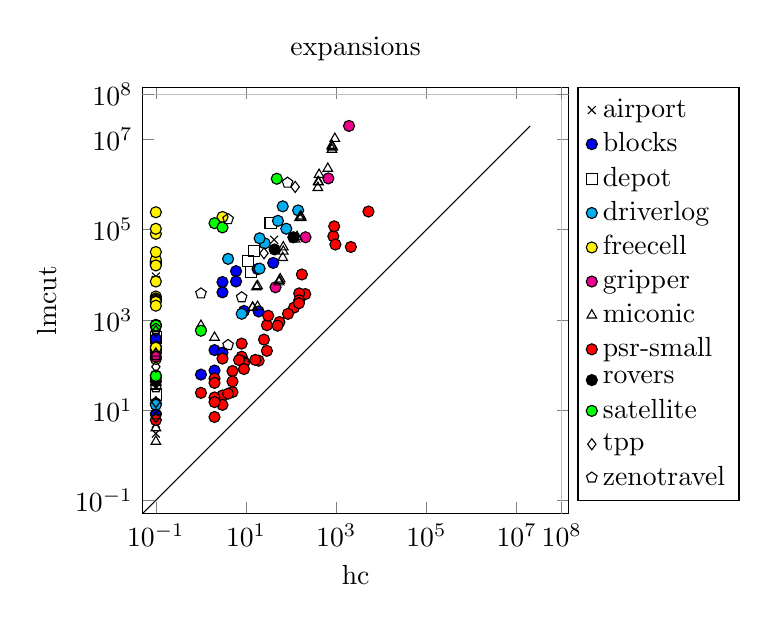
\begin{tikzpicture}
\begin{axis}[extra x tick style={grid=major}, extra x ticks=100000000, extra y tick style={grid=major}, extra y ticks=100000000, 
height=7.00cm, legend cell align=left, legend style={at={(1.4, 1)}}, title=expansions, width=7.00cm, xlabel=hc, xmin=0.05, xmode=log, ylabel=lmcut, ymin=0.05, ymode=log]
\addplot[color=green, mark=x, mark options={{draw=black}}, only marks] coordinates {
(0.100000, 33) (0.100000, 219) (0.100000, 181) (42, 59492) (0.100000, 217) (0.100000, 6) (0.100000, 9131) (0.100000, 5) (0.100000, 7615) (0.100000, 7625) (0.100000, 245) (0.100000, 3) (0.100000, 8)
};
\addlegendentry{airport}
\addplot[color=blue, mark=*, mark options={{draw=black}}, only marks] coordinates {
(18, 13376) (0.100000, 187) (2, 213) (6, 12007) (0.100000, 58) (6, 7076) (9, 1570) (0.100000, 14) (19, 1532) (3, 4066) (2, 75) (0.100000, 379) (3, 6886) (40, 18268) (1, 61) (0.100000, 8) (3, 187)
};
\addlegendentry{blocks}
\addplot[color=magenta, mark=square, mark options={{draw=black}}, only marks] coordinates {
(0.100000, 22) (15, 34039) (11, 20162) (35, 142452) (13, 11292) (0.100000, 407)
};
\addlegendentry{depot}
\addplot[color=cyan, mark=*, mark options={{draw=black}}, only marks] coordinates {
(0.100000, 16896) (26, 49620) (20, 64248) (51, 156560) (0.100000, 13) (143, 266848) (4, 22448) (65, 328115) (20, 13650) (8, 1360) (78, 104720)
};
\addlegendentry{driverlog}
\addplot[color=yellow, mark=*, mark options={{draw=black}}, only marks] coordinates {
(0.100000, 17761) (0.100000, 3286) (0.100000, 2971) (0.100000, 7067) (0.100000, 19591) (0.100000, 242704) (0.100000, 19141) (0.100000, 21631) (0.100000, 226) (0.100000, 136) (0.100000, 211) (0.100000, 2791) (3, 190470) (0.100000, 2626) (0.100000, 256) (0.100000, 16051) (0.100000, 241) (0.100000, 2506) (0.100000, 80809) (0.100000, 2056) (0.100000, 31823) (0.100000, 766) (0.100000, 104311)
};
\addlegendentry{freecell}
\addplot[color=magenta, mark=*, mark options={{draw=black}}, only marks] coordinates {
(1920, 19916814) (45, 5268) (208, 67710) (0.100000, 151) (668, 1367176)
};
\addlegendentry{gripper}
\addplot[color=cyan, mark=triangle, mark options={{draw=black}}, only marks] coordinates {
(55, 7443) (0.100000, 181) (135, 69039) (155, 185047) (18, 5647) (819, 6915236) (156, 182083) (0.100000, 43) (2, 406) (395, 1143604) (409, 1131564) (17, 5356) (824, 6718966) (803, 5972930) (54, 6872) (18, 1954) (14, 1892) (416, 1656749) (0.100000, 50) (67, 40958) (0.100000, 4) (122, 60879) (57, 8012) (65, 23797) (166, 185293) (391, 846923) (931, 10411953) (649, 2261005) (14, 1861) (801, 7337121) (164, 198138) (1, 745) (0.100000, 2) (67, 32915)
};
\addlegendentry{miconic}
\addplot[color=red, mark=*, mark options={{draw=black}}, only marks] coordinates {
(5, 73) (206, 3719) (863, 71216) (902, 118208) (3, 21) (29, 760) (8, 152) (19, 124) (958, 46688) (9, 116) (116, 1866) (55, 892) (151, 3851) (3, 138) (31, 1232) (25, 364) (8, 297) (5, 25) (4, 23) (0.100000, 772) (9, 109) (173, 10124) (3, 13) (2109, 41214) (29, 205) (5183, 251714) (85, 1355) (1, 24) (2, 19) (2, 7) (151, 2707) (7, 128) (2, 50) (2, 40) (5, 43) (16, 129) (0.100000, 6) (9, 81) (2, 15) (50, 741) (149, 2328)
};
\addlegendentry{psr-small}
\addplot[color=black, mark=*, mark options={{draw=black}}, only marks] coordinates {
(43, 36383) (0.100000, 43) (0.100000, 50) (112, 67588)
};
\addlegendentry{rovers}
\addplot[color=green, mark=*, mark options={{draw=black}}, only marks] coordinates {
(0.100000, 57) (2, 138858) (48, 1342395) (0.100000, 745) (1, 573) (3, 112017)
};
\addlegendentry{satellite}
\addplot[color=blue, mark=diamond, mark options={{draw=black}}, only marks] coordinates {
(0.100000, 91) (0.100000, 15) (0.100000, 559) (0.100000, 7) (25, 29953) (123, 884427)
};
\addlegendentry{tpp}
\addplot[color=red, mark=pentagon, mark options={{draw=black}}, only marks] coordinates {
(0.100000, 8) (0.100000, 632) (1, 3844) (0.100000, 166) (4, 170892) (8, 3160) (83, 1096013) (0.100000, 32) (4, 276)
};
\addlegendentry{zenotravel}
\addplot[color=black] coordinates {(0.050000, 0.050000) (19916814, 19916814)};
\end{axis}
\end{tikzpicture}
\\
        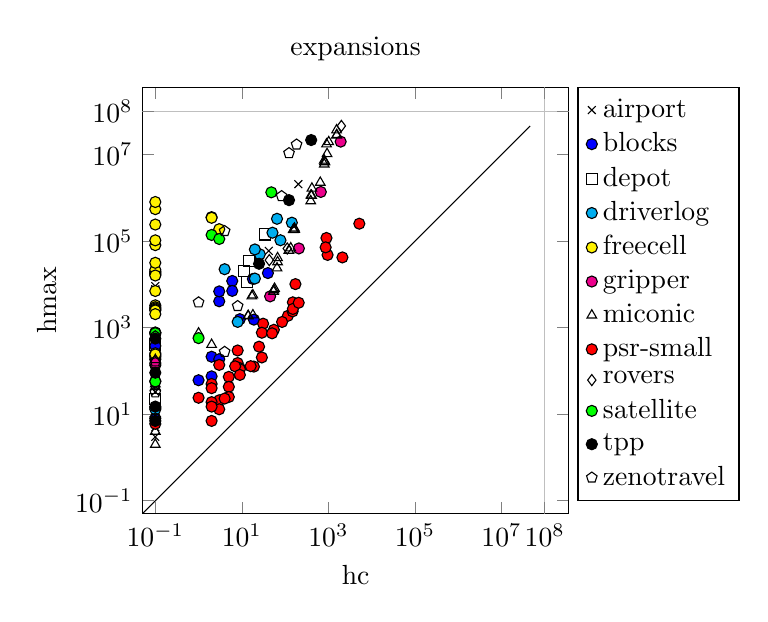
\begin{tikzpicture}
\begin{axis}[extra x tick style={grid=major}, extra x ticks=100000000, extra y tick style={grid=major}, extra y ticks=100000000, 
height=7.00cm, legend cell align=left, legend style={at={(1.4, 1)}}, title=expansions, width=7.00cm, xlabel=hc, xmin=0.05, xmode=log, ylabel=hmax, ymin=0.05, ymode=log]
\addplot[color=green, mark=x, mark options={{draw=black}}, only marks] coordinates {
(42, 59583) (0.100000, 33) (0.100000, 219) (0.100000, 181) (0.100000, 6) (0.100000, 217) (0.100000, 245) (202, 2073240) (0.100000, 9131) (0.100000, 5) (0.100000, 7615) (0.100000, 7625) (0.100000, 3) (0.100000, 8)
};
\addlegendentry{airport}
\addplot[color=blue, mark=*, mark options={{draw=black}}, only marks] coordinates {
(9, 1572) (18, 13376) (0.100000, 379) (6, 12007) (0.100000, 58) (6, 7076) (0.100000, 14) (2, 213) (3, 4066) (2, 75) (0.100000, 187) (40, 18270) (3, 6886) (1, 61) (0.100000, 8) (3, 187) (19, 1534)
};
\addlegendentry{blocks}
\addplot[color=magenta, mark=square, mark options={{draw=black}}, only marks] coordinates {
(0.100000, 22) (35, 142466) (13, 11292) (11, 20161) (15, 34032) (0.100000, 407)
};
\addlegendentry{depot}
\addplot[color=cyan, mark=*, mark options={{draw=black}}, only marks] coordinates {
(0.100000, 16896) (26, 49620) (20, 64248) (51, 156560) (0.100000, 13) (143, 266816) (4, 22448) (20, 13650) (8, 1360) (65, 328078) (78, 104720)
};
\addlegendentry{driverlog}
\addplot[color=yellow, mark=*, mark options={{draw=black}}, only marks] coordinates {
(0.100000, 17761) (0.100000, 3286) (0.100000, 2971) (0.100000, 19591) (2, 357856) (0.100000, 19141) (0.100000, 548746) (0.100000, 21631) (0.100000, 226) (0.100000, 136) (0.100000, 802036) (0.100000, 211) (0.100000, 2791) (0.100000, 31561) (0.100000, 2626) (0.100000, 7036) (0.100000, 256) (0.100000, 16051) (0.100000, 241) (0.100000, 80806) (0.100000, 2506) (0.100000, 2056) (2, 346276) (3, 188791) (0.100000, 766) (0.100000, 104311) (0.100000, 241546)
};
\addlegendentry{freecell}
\addplot[color=magenta, mark=*, mark options={{draw=black}}, only marks] coordinates {
(1920, 19918398) (668, 1368076) (208, 67738) (0.100000, 151) (45, 5283)
};
\addlegendentry{gripper}
\addplot[color=cyan, mark=triangle, mark options={{draw=black}}, only marks] coordinates {
(395, 1143601) (0.100000, 181) (18, 5647) (409, 1131640) (0.100000, 43) (801, 7341225) (17, 5356) (1563, 28711853) (67, 40955) (391, 846921) (931, 10420707) (18, 1954) (803, 5975018) (55, 7441) (0.100000, 50) (907, 17460317) (122, 60875) (1019, 19611126) (156, 182080) (166, 185292) (819, 6917972) (155, 185045) (1542, 36749162) (65, 23798) (54, 6870) (824, 6722843) (0.100000, 4) (1545, 27889713) (649, 2261740) (14, 1861) (416, 1656947) (67, 32916) (57, 8012) (2, 406) (1, 745) (14, 1892) (164, 198133) (135, 69035) (0.100000, 2)
};
\addlegendentry{miconic}
\addplot[color=red, mark=*, mark options={{draw=black}}, only marks] coordinates {
(116, 1880) (5, 73) (902, 118208) (3, 21) (173, 10156) (8, 152) (2, 19) (9, 116) (5, 43) (55, 892) (151, 3851) (3, 138) (25, 364) (8, 297) (5, 25) (4, 23) (149, 2378) (5183, 252962) (0.100000, 772) (31, 1236) (958, 47992) (9, 109) (1, 24) (3, 13) (29, 764) (2109, 42030) (29, 205) (85, 1355) (19, 126) (2, 7) (151, 2707) (7, 128) (2, 50) (863, 71716) (2, 40) (16, 129) (0.100000, 6) (206, 3759) (9, 81) (2, 15) (50, 741)
};
\addlegendentry{psr-small}
\addplot[color=blue, mark=diamond, mark options={{draw=black}}, only marks] coordinates {
(0.100000, 43) (112, 67588) (43, 36387) (1997, 45935775) (0.100000, 50)
};
\addlegendentry{rovers}
\addplot[color=green, mark=*, mark options={{draw=black}}, only marks] coordinates {
(0.100000, 57) (48, 1342391) (2, 138858) (0.100000, 745) (1, 573) (3, 112017)
};
\addlegendentry{satellite}
\addplot[color=black, mark=*, mark options={{draw=black}}, only marks] coordinates {
(0.100000, 91) (0.100000, 559) (0.100000, 15) (400, 21653693) (0.100000, 7) (123, 884552) (25, 29955)
};
\addlegendentry{tpp}
\addplot[color=red, mark=pentagon, mark options={{draw=black}}, only marks] coordinates {
(0.100000, 8) (123, 10801620) (83, 1096038) (8, 3160) (0.100000, 632) (1, 3844) (0.100000, 166) (4, 170892) (0.100000, 32) (4, 276) (184, 17075893)
};
\addlegendentry{zenotravel}
\addplot[color=black] coordinates {(0.050000, 0.050000) (45935775, 45935775)};
\end{axis}
\end{tikzpicture}

    \end{center}
   